\documentclass[compress]{beamer}




%%%%%%%%%%%%%%%%%%%%%%%%%%%
% LaTeX package inclusion %
%%%%%%%%%%%%%%%%%%%%%%%%%%%
\usepackage{times}
\usepackage{units}
\usepackage{mathrsfs}
\usepackage{diss} % defines \bv and some other stuff
\usepackage{subfigure}
\usepackage{multirow}
\usepackage{amsmath}
\usepackage{amssymb}
%\usepackage{algorithm}
%\usepackage{algorithmic}
\usepackage{hyperref}
\usepackage{listings}
\usepackage{movie15}
\usepackage{stmaryrd} % \llbracket
\graphicspath{{figs/}}



\usefonttheme[
  onlymath
]{serif} %onlymath option doesn't look too bad, eqns are more readable this way.

\definecolor{DarkGreen}{rgb}{0.13,0.55,0.13}
\definecolor{DarkRed}{rgb}{0.55,0.13,0.13}
\definecolor{mygray}{rgb}{0.5,0.5,0.5}
\definecolor{mymauve}{rgb}{0.58,0,0.82}
\setcounter{tocdepth}{1}


\usetheme{UB}
%\usetheme{nasatalk}

\definecolor{nasablue}{RGB}{0,96,169}
\definecolor{nasared}{RGB}{239,61,66}
\definecolor{orionblue}{RGB}{15,16,64}

%\usecolortheme{orchid} % white on dark block titles.  use w/ whale.
%\usecolortheme{whale} % darkest top titles, usually used by CFDLab presenters
\setbeamertemplate{itemize items}[circle]% Force any theme (eg Antibes) to use circle bullets
%\useinnertheme[shadow]{rounded} % Causes itemize blocks to have rounded corners & drop shadows
%\logo{\includegraphics[width=.5in]{common/rawfigs/word3}}
%\setbeamercolor{title}{fg=red!80!black,bg=red!20!white} %pink title!

\title[The \texttt{libMesh} Finite Element Library]{The \texttt{libMesh} Finite Element Library \\ \vspace{.5em} \emph{\large Object-Oriented High-Performance Computing}}
\author[P.~T.~Bauman]{Paul T. Bauman}
\institute[UB]{University at Buffalo, SUNY}
\date{March 25, 2015}

%\AtBeginSection[]{\frame{\tableofcontents[current]}}

% Dr. Carey's Notes:
% I had in mind some of the material we have in the Libmesh papers well
% as  from the perspective of:(1) a very knowlegable  developer,(2)
% installing an application with experience (3)  applying an
% application for parametric runs  with some examples. perhaps some of
% the issues encounter, as in all such codes like stopping criteria for
% adaptive refinement, selection of error indicators, flexibility in
% model adaption, ( adding terms, modifying constitutive models etc).
% perhaps something on the coarsening /refining ; one level exceptions
% etc. it would be helpful if you, Ben and Roy coordinated this.
% Someone should talk about PETSc, partitioning etc. Someone about
% memory restrictions etc. Strengths and limitations.  examples, couple
% of movies etc etc


% Abstract:
% This talk will focus on several of the practical aspects involved in
% using the LibMesh library for finite element analysis.  The topics
% covered will include: the steps in going from a mathematical model
% (PDE) to a working implementation (code), stopping criteria for
% adaptive refinement, the selection of error indicators, and model
% adaptation (adding terms, changing constitutive laws, etc).  The
% strengths, weaknesses, and current limitations of the library will
% be discussed in the same practical context.  Finally, some additional
% examples giving a flavor of the types of applications which have
% already been developed around the library will be given.
%\setbeamercovered{transparent}


\newcommand{\R}{\mathscr{R}}
\newcommand{\LibMesh}{\texttt{libMesh}}
\newcommand{\libmesh}{\texttt{libMesh}}
\newcommand{\emphcolor}[1]{\textcolor{nasablue}{#1}}
\newcommand{\royslide}[2]{\begin{frame} \frametitle{#1} #2 \end{frame}}
\newcommand{\royitemizebegin}[1]{\begin{block}{#1} \begin{itemize}}
\newcommand{\royitemizeend}{\end{itemize} \end{block}}

\begin{document}

\lstset{
  language=C++,
  basicstyle=\scriptsize\ttfamily,
  frame=none,
  commentstyle=\color{nasared},
  keywordstyle=\color{nasablue},   % keyword style
  numbers=none,                    % where to put the line-numbers; possible values are (none, left, right)
  numbersep=3pt,                   % how far the line-numbers are from the code
  numberstyle=\tiny\color{mygray}, % the style that is used for the line-numbers
  rulecolor=\color{black},         % if not set, the frame-color may be changed on line-breaks within not-black text
  showspaces=false,                % show spaces everywhere adding particular underscores; it overrides 'showstringspaces'
  showstringspaces=false,          % underline spaces within strings only
  showtabs=false,                  % show tabs within strings adding particular underscores
  stepnumber=2,                    % the step between two line-numbers. If it's 1, each line will be numbered
  stringstyle=\color{mymauve}      % string literal style
}


\begin{frame}
  \titlepage
\end{frame}



%===============================================================================
% Objectives
%===============================================================================
\begin{frame}
\frametitle{Course Objectives}

\begin{block}{Scope}
\begin{itemize}
\item Overview of libMesh:
        \begin{itemize}
        \item geometry data structures
        \item finite element data structures
        \item Building programs to solve finite element formulations
        \end{itemize}
\item Survey of more advanced features of library, if time
\end{itemize}
\end{block}

\begin{block}{Target Audience}
\begin{itemize}
\item PhD students/Postdocs with some knowledge of C++ and finite
  element methods
\end{itemize}
\end{block}

\begin{block}{Slides}
\begin{itemize}
\item Slides will be publicly available at: \url{https://github.com/libMesh/Documents}
\end{itemize}
\end{block}

\end{frame}

%===============================================================================
% Course Notes
%===============================================================================
\begin{frame}
\frametitle{Course Notes}

\begin{block}{This is for you!}
\begin{itemize}
\item Please stop me to ask questions
\item Please stop me to have a discussion
\item Please download the slides at your convenience
\end{itemize}
\end{block}

\begin{block}{Online Resources}
\begin{itemize}
\item \url{https://libmesh.github.io}
\item \href{mailto:libmesh-users@lists.sourceforge.net}{libmesh-users@lists.sourceforge.net}
\item \href{mailto:libmesh-devel@lists.sourceforge.net}{libmesh-devel@lists.sourceforge.net}
\item \textbf{PLEASE} don't email me directly about \texttt{libMesh}, use the list!
\end{itemize}
\end{block}

\end{frame}

%\begin{frame}
%  \frametitle{Originators of \texttt{libMesh}}
%  \begin{block}{}
%    \begin{itemize}
%    \item 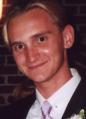
\includegraphics[scale=3]{benkirk} Benjamin S. Kirk, NASA Johnson Space Center
%    \item 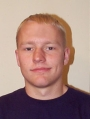
\includegraphics[scale=0.35]{jwpeterson} John W. Peterson, Idaho National Lab
%    \item 
\includegraphics[scale=0.35]{roystgnr} Roy H. Stogner, University of Texas at Austin
%    \end{itemize}
%  \end{block}
%
%\end{frame}

\frame
{
  \frametitle{Thanks to Dr.\ Graham F.\ Carey}

  \begin{columns}
    \begin{column}{.55\textwidth}
      \scriptsize
      \begin{quote}
        The original development team was heavily influenced by Professor Graham F. Carey, professor of aerospace engineering and engineering mechanics at The University of Texas at Austin, director of the ICES Computational Fluid Dynamics Laboratory, and holder of the Richard B. Curran Chair in Engineering.

        Many of the technologies employed in libMesh were implemented because Dr. Carey taught them to us, we went back to the lab, and immediately began coding. In a very real way, he was ultimately responsible for this library that we hope you may find useful, despite his continued insistence that ``no one ever got a PhD from here for writing a code.''
      \end{quote}
\normalsize
    \end{column}
    \begin{column}{.45\textwidth}
      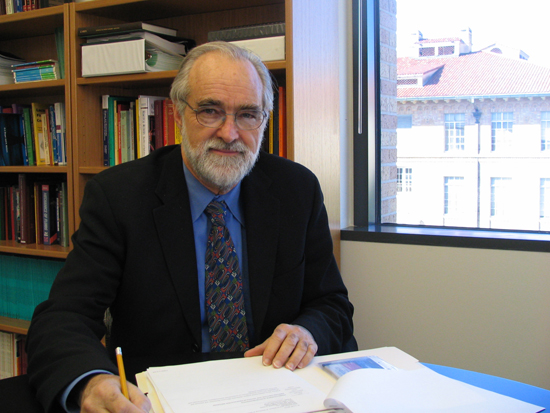
\includegraphics[width=\textwidth]{grahamcarey}
    \end{column}
  \end{columns}
}

% The optional argument [<+->] means everything on the frame will be displayed incrementally.


\begin{frame}[shrink]
  \begin{block}{Major Code Contributors}
    \scriptsize
    \begin{center}
      \begin{tabular}{|l|l|} \hline
        Benjamin S. Kirk & benkirk \\
        Bill Barth       & bbarth \\
        Cody Permann     & permcody \\
        Daniel Dreyer    & ddreyer \\
        David Andrs      & andrsd \\
        David Knezevic   & knezed01 \\
        Derek Gaston     & friedmud \\
        Dmitry Karpeev   & karpeev \\
        Florian Prill    & fprill \\
        Jason Hales      & jasondhales \\
        John W. Peterson & jwpeterson \\
        Paul T. Bauman   & pbauman \\
        Roy H. Stogner   & roystgnr \\
        Steffen Petersen & spetersen \\
        Sylvain Vallaghe & svallagh \\
        Tim Kroeger      & sheep\_tk \\
        Truman Ellis     & trumanellis \\
        Wout Ruijter     & woutruijter \\ \hline
      \end{tabular}
    \end{center}
    \begin{itemize}
      \item Thanks to Wolfgang Bangerth and the \texttt{deal.II} team for initial technical inspiration.
      \item Also, thanks to Jed Brown, Robert McLay, \& many others for discussions over the years.
    \end{itemize}
  \end{block}
\end{frame}


%%%%%%%%%%%%%%%%%%%%%%%%%%%%%%%%%%%%%%%%%%%%%%%%%%%%%%%%%%%%%%%%%%%%%
\royslide{Outline}{
\begin{columns}
\begin{column}{.55\textwidth}
  \tableofcontents
\end{column}
\begin{column}{.45\textwidth}
  \includegraphics[width=\textwidth]{parallelism/thinmesh}
\end{column}
\end{columns}
}

%\subsection*{Non-Trivial Applications}
\begin{frame}%[t]
%  \frametitle{Weighted Residual Connection}
  %\begin{block}{}
  \begin{itemize}%[<+->]
  \item{\libMesh{} provides several of the tools necessary to construct
    these systems, but it is not specifically written to solve any one
    problem.}

  \item{First, a few of the non-trivial applications which have been built on
    top of the library.}
    
%%   \item{In each case, the matrix $A$ is the ``Jacobian''
%%     operator, and the right-hand side vector $b$ is the
%%     weighted residual itself.}

    %% 	\item{This is true even in the case of linear $\R( u )$, since
    %% 	  in this case the linearized operator is
    %% 	  \begin{eqnarray}
    %% 	    \nonumber
    %% 	    \R'( u )w &:=& \lim_{\varepsilon\rightarrow 0}
    %% 	    \frac{\R(u+\varepsilon w) - \R(u)}{\varepsilon} \\
    %% 	    \nonumber
    %% 	    &=& \R(w)
    %% 	  \end{eqnarray}
    %% 	}
  \end{itemize}
%\end{block}
\end{frame}	  

%\subsection*{Natural Convection}
\begin{frame}[t]
  \begin{center}
    \includegraphics[width=.45\textwidth]{part_trans}
    %\\
    \includegraphics[width=.45\textwidth]{streamtraces}
  \end{center}
  \begin{block}{}
    \begin{itemize}
    \item{
      Tetrahedral mesh of ``pipe'' geometry.
      Stream ribbons colored by temperature.
      }
      \end{itemize}
  \end{block}
\end{frame}

%\subsection*{Surface-Tension-Driven Flow}
\begin{frame}[t]
  \begin{center}
    \includegraphics[width=.6\textwidth]{rbm_adapt_soln}    
  \end{center}

  \begin{block}{}
    \begin{itemize}
    \item{Adaptive grid solution shown
      with temperature contours and velocity vectors.
      }
      \end{itemize}
  \end{block}
\end{frame}

%\subsection*{Double-Diffusive Convection}
\begin{frame}[t]
  \begin{center}
    \includegraphics[width=.6\textwidth]{dd}    
  \end{center}

  \begin{block}{}
    \begin{itemize}
    \item{Solute contours: a plume of
      warm, low-salinity fluid is convected upward through a porous medium.
      }
      \end{itemize}
  \end{block}
\end{frame}



%\subsection*{Tumor Angiogenesis}
\begin{frame}[t]
  \begin{center}
    \includegraphics[width=.6\textwidth]{tumor_model}    
  \end{center}

  \begin{block}{}
    \begin{itemize}
    \item{%Tumor angiogenesis model simulation.
      The tumor secretes
      a chemical which stimulates blood vessel formation.
      }
      \end{itemize}
  \end{block}
\end{frame}



%\subsection*{Phase Separation}
\begin{frame}[t]
  \begin{center}
    \includegraphics[width=.3\textwidth]{ch3D02-006}    
    \includegraphics[width=.3\textwidth]{ch3D02-024}    
    \includegraphics[width=.3\textwidth]{ch3D02-096}    
  \end{center}

  \begin{block}{}
    \begin{itemize}
    \item{%Tumor angiogenesis model simulation.
      Directed pattern self-assembly in spinodal decomposition of binary
mixture
      }
      \end{itemize}
  \end{block}
\end{frame}



%\subsection*{Compressible Flow}

\frame
{
  \frametitle{Compressible Shocked Flow}
  \begin{itemize}[<+->]
    \item Original compressible flow code written by Ben Kirk utilizing \libMesh{}.
      \begin{itemize}[<+->]
      \item Solves both Compressible Navier Stokes and Inviscid Euler.
      \item Includes both SUPG and a shock capturing scheme.
      \end{itemize}
    \item Original redistribution code written by Larisa Branets.
      \begin{itemize}[<+->]
      \item Simultaneous optimization of element shape and size.
      \item Directable via user supplied error estimate.
      \end{itemize}
    \item Integration work done by Derek Gaston.
      \begin{itemize}[<+->]
      \item Combination of redistribution, $h$ refinement.
      \item Applicable to other problem classes.
      \end{itemize}
  \end{itemize}
}

\frame
{
  \frametitle{Problem Specification}
  \begin{itemize}[<+->]
    \item The problem studied is that of an oblique shock generated by a $10^o$ wedge angle. 
      \begin{itemize}[<+->]
      \item This problem has an exact solution for density which is a step function.
      \item Utilizing \libMesh{}'s exact solution capability the exact
$L_2$ error can be solved for.
      \item The exact solution is shown below:
        \begin{figure}
          \begin{center}
            \includegraphics[viewport=20 10 660 600,clip=true,width=.4\textwidth]{shock.pdf}
          \end{center}
        \end{figure}
    \end{itemize}
  \end{itemize}
}

\frame
{
  \frametitle{Uniformly Refined Solutions}
  \begin{itemize}[<+->]
  \item For comparison purposes, here is a mesh and a solution after 1 uniform refinement with 10890 DOFs.
    \begin{figure}[!htb]
      \begin{center}
        \subfigure[Mesh after 1 uniform refinement.]{\label{fig:fob_uniform_2_mesh}\includegraphics[viewport=110 30 600 550,clip=true,width=.42\textwidth]{fob_uniform_2_mesh.pdf}}
        \subfigure[Solution after 1 uniform refinement.]{\label{fig:fob_uniform_2_sol}\includegraphics[viewport=110 30 600 520,clip=true,width=.42\textwidth]{fob_uniform_2_sol.pdf}}
      \end{center}
    \end{figure}
  \end{itemize}
}

\frame
{
  \frametitle{H-Adapted Solutions}
  \begin{itemize}[<+->]
    \item A flux jump indicator was employed as the error indcator along with a statistical flagging scheme.
    \item Here is a mesh and solution after 2 adaptive refinements containing 10800 DOFs:
      \begin{figure}[!htb]
        \begin{center}
          \subfigure[Mesh, 2 refinements]{\label{fig:fob_adapt_3_mesh}\includegraphics[viewport=110 30 600 550,clip=true,width=.42\textwidth]{fob_adapt_3_mesh.pdf}}
          \subfigure[Solution]{\label{fig:fob_adapt_3_sol}\includegraphics[viewport=110 30 600 520,clip=true,width=.42\textwidth]{fob_adapt_3_sol.pdf}}
        \end{center}
      \end{figure}
  \end{itemize}
}

\frame
{
  \frametitle{Redistributed Solutions}
  \begin{itemize}[<+->]
    \item Redistribution utilizing the same flux jump indicator.
      \begin{figure}[!htb]
        \begin{center}
          \subfigure[Mesh, 8 redistribution steps]{\label{fig:fob_redist_adapt_8_mesh}\includegraphics[viewport=110 30 600 550,clip=true,width=.42\textwidth]{fob_redist_adapt_8_mesh.pdf}}
          \subfigure[Solution]{\label{fig:fob_redist_adapt_8_sol}\includegraphics[viewport=110 30 600 520,clip=true,width=.42\textwidth]{fob_redist_adapt_8_sol.pdf}}
        \end{center}
      \end{figure}
  \end{itemize}
}

\frame
{
  \frametitle{Redistributed and Adapted}
  \begin{itemize}[<+->]
    \item Now combining the two, here are the mesh and solution after 2 adaptations beyond the previous redistribution containing 10190 DOFs.
      \begin{figure}[!htb]
        \begin{center}
          \subfigure[Mesh, 2 refinements]{\label{fig:fob_redist_adapt_10_mesh}\includegraphics[viewport=110 30 600 550,clip=true,width=.42\textwidth]{fob_redist_adapt_10_mesh.pdf}}
          \subfigure[Solution]{\label{fig:fob_redist_adapt_10_sol}\includegraphics[viewport=110 30 600 520,clip=true,width=.42\textwidth]{fob_redist_adapt_10_sol.pdf}}
        \end{center}
      \end{figure}
  \end{itemize}
}

\frame
{
  \frametitle{Solution Comparison}
  \begin{itemize}[<+->]
    \item For a better comparison here are 3 of the solutions, each with around 11000 DOFs:
      \begin{figure}[!htb]
        \begin{center}
          \subfigure[Uniform.]{\label{fig:fob_uniform_2_sol}\includegraphics[viewport=110 30 600 520,clip=true,width=.3\textwidth]{fob_uniform_2_sol.pdf}}
          \subfigure[Adaptive.]{\label{fig:fob_adapt_3_sol}\includegraphics[viewport=110 30 600 520,clip=true,width=.3\textwidth]{fob_adapt_3_sol.pdf}}
          \subfigure[R + H.]{\label{fig:fob_redist_adapt_10_sol}\includegraphics[viewport=110 30 600 520,clip=true,width=.3\textwidth]{fob_redist_adapt_10_sol.pdf}}
        \end{center}
      \end{figure}
  \end{itemize}
}

\frame
{
  \frametitle{Error Plot}
  \begin{itemize}[<+->]
    \item \libMesh{} provides capability for computing error norms against an exact solution.
    \item The exact solution is not in $H^1$ therefore we only obtain
the $L_2$ convergence plot:
      \begin{figure}[!htb]
      \begin{center}
        \subfigure[LogLog plot of L2 vs DOFs.]{\label{fig:fob_l2}\includegraphics[viewport=0 10 600 400,clip=true,width=.7\textwidth]{fob_l2.pdf}}
      \end{center}
      \end{figure}
  \end{itemize}
}

\frame
{
  %\frametitle{Other Compressible Flow Examples}
    \begin{figure}[!htb]
      \begin{center}
        \subfigure{\label{fig:fob_uniform_2_sol}\includegraphics[width=.4\textwidth]{Hypersonic_cow_mach}}
        \subfigure{\label{fig:fob_adapt_3_sol}\includegraphics[width=.4\textwidth]{Benkirk_orbiter_reentry_side_view}}
        \subfigure{\label{fig:fob_redist_adapt_10_sol}\includegraphics[width=.4\textwidth]{Benkirk_schlieren}}
        \subfigure{\label{fig:fob_redist_adapt_10_sol}\includegraphics[width=.4\textwidth]{Benkirk_double_cone_M}}
      \end{center}
    \end{figure}
}

\section{Application Examples}
\subsection{Application Results}



%%%%%%%%%%%%%%%%%%%%%%%%%%%%%%%%%%%%%%%%%%%%%%%%%
\frame
{
  \frametitle{FIN-S: Fully Implicit Navier-Stokes}

  \begin{columns}
    \begin{column}{0.45\textwidth}
      \begin{itemize}
      \item Kirk, Stogner, Bauman, Oliver, Computers \& Fluids, 2014
      \item Application for high-speed (including reentry)
        compressible flows in thermochemical nonequilibrium
      \item Including AMR capabilities
      \item Fully implicit coupling with surface response models
      \end{itemize}
    \end{column}
    %
    \begin{column}{0.45\textwidth}
      \begin{center}
        \only<1>{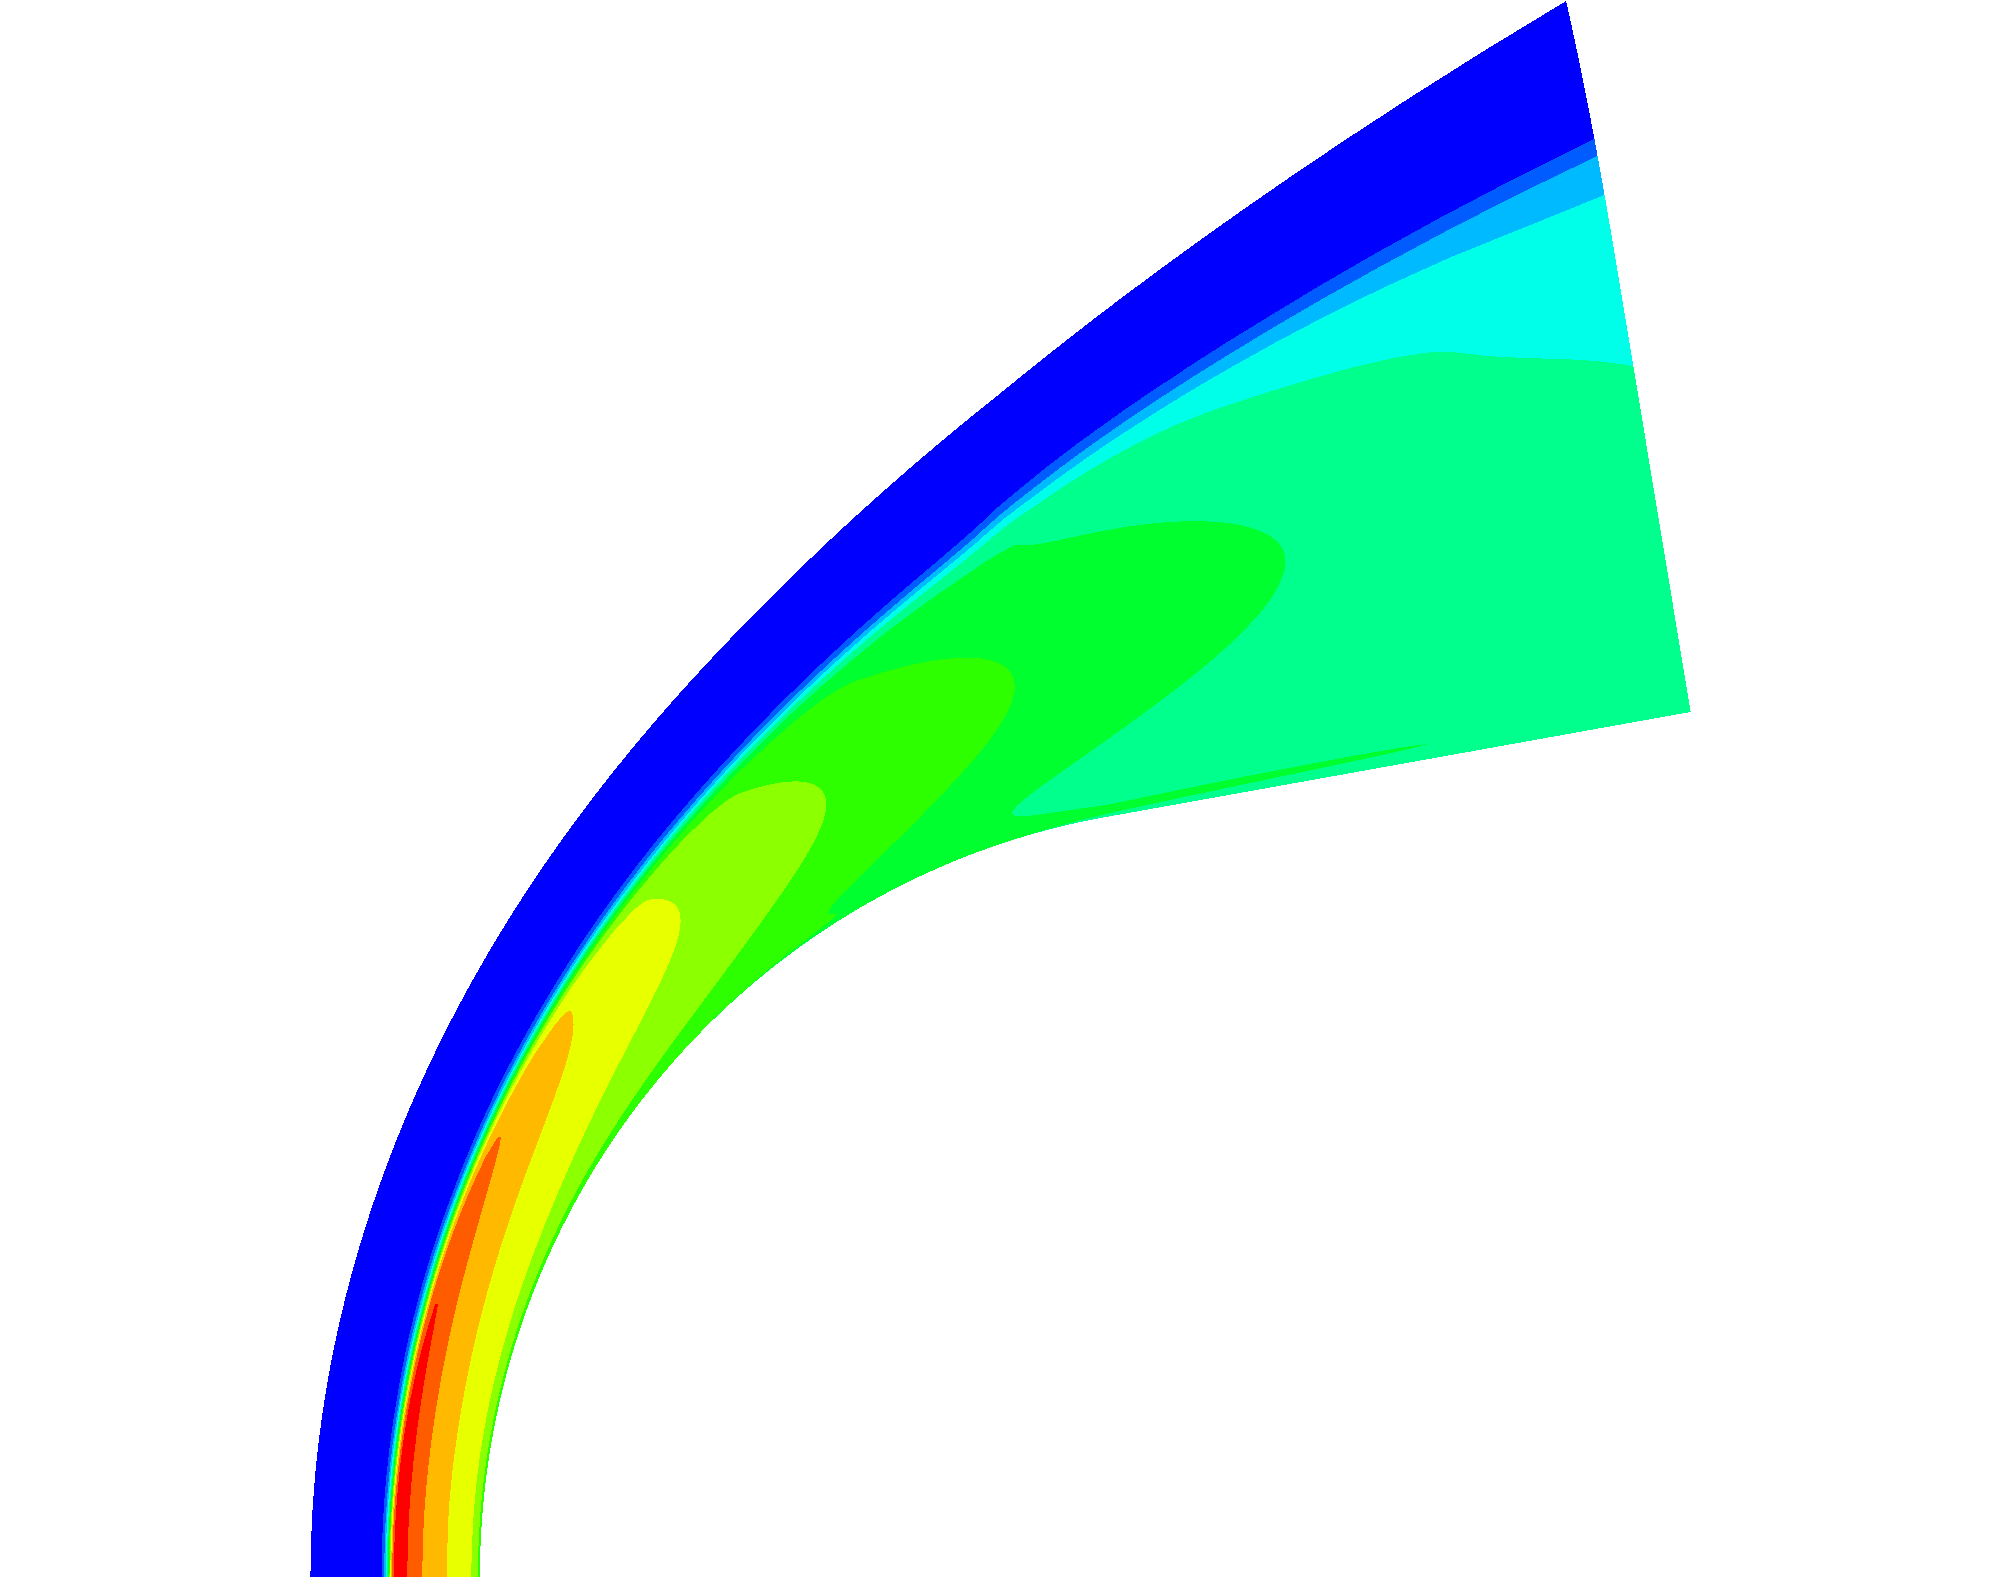
\includegraphics[height=\linewidth]{nosetip/smeared.png}}
        \only<2>{\includegraphics[height=\linewidth]{nosetip/amr.png}}
        \only<3>{\includegraphics[height=\linewidth]{nosetip/smeared.pdf}}
        \only<4>{\includegraphics[height=\linewidth]{nosetip/amr.pdf}}
        \only<5>{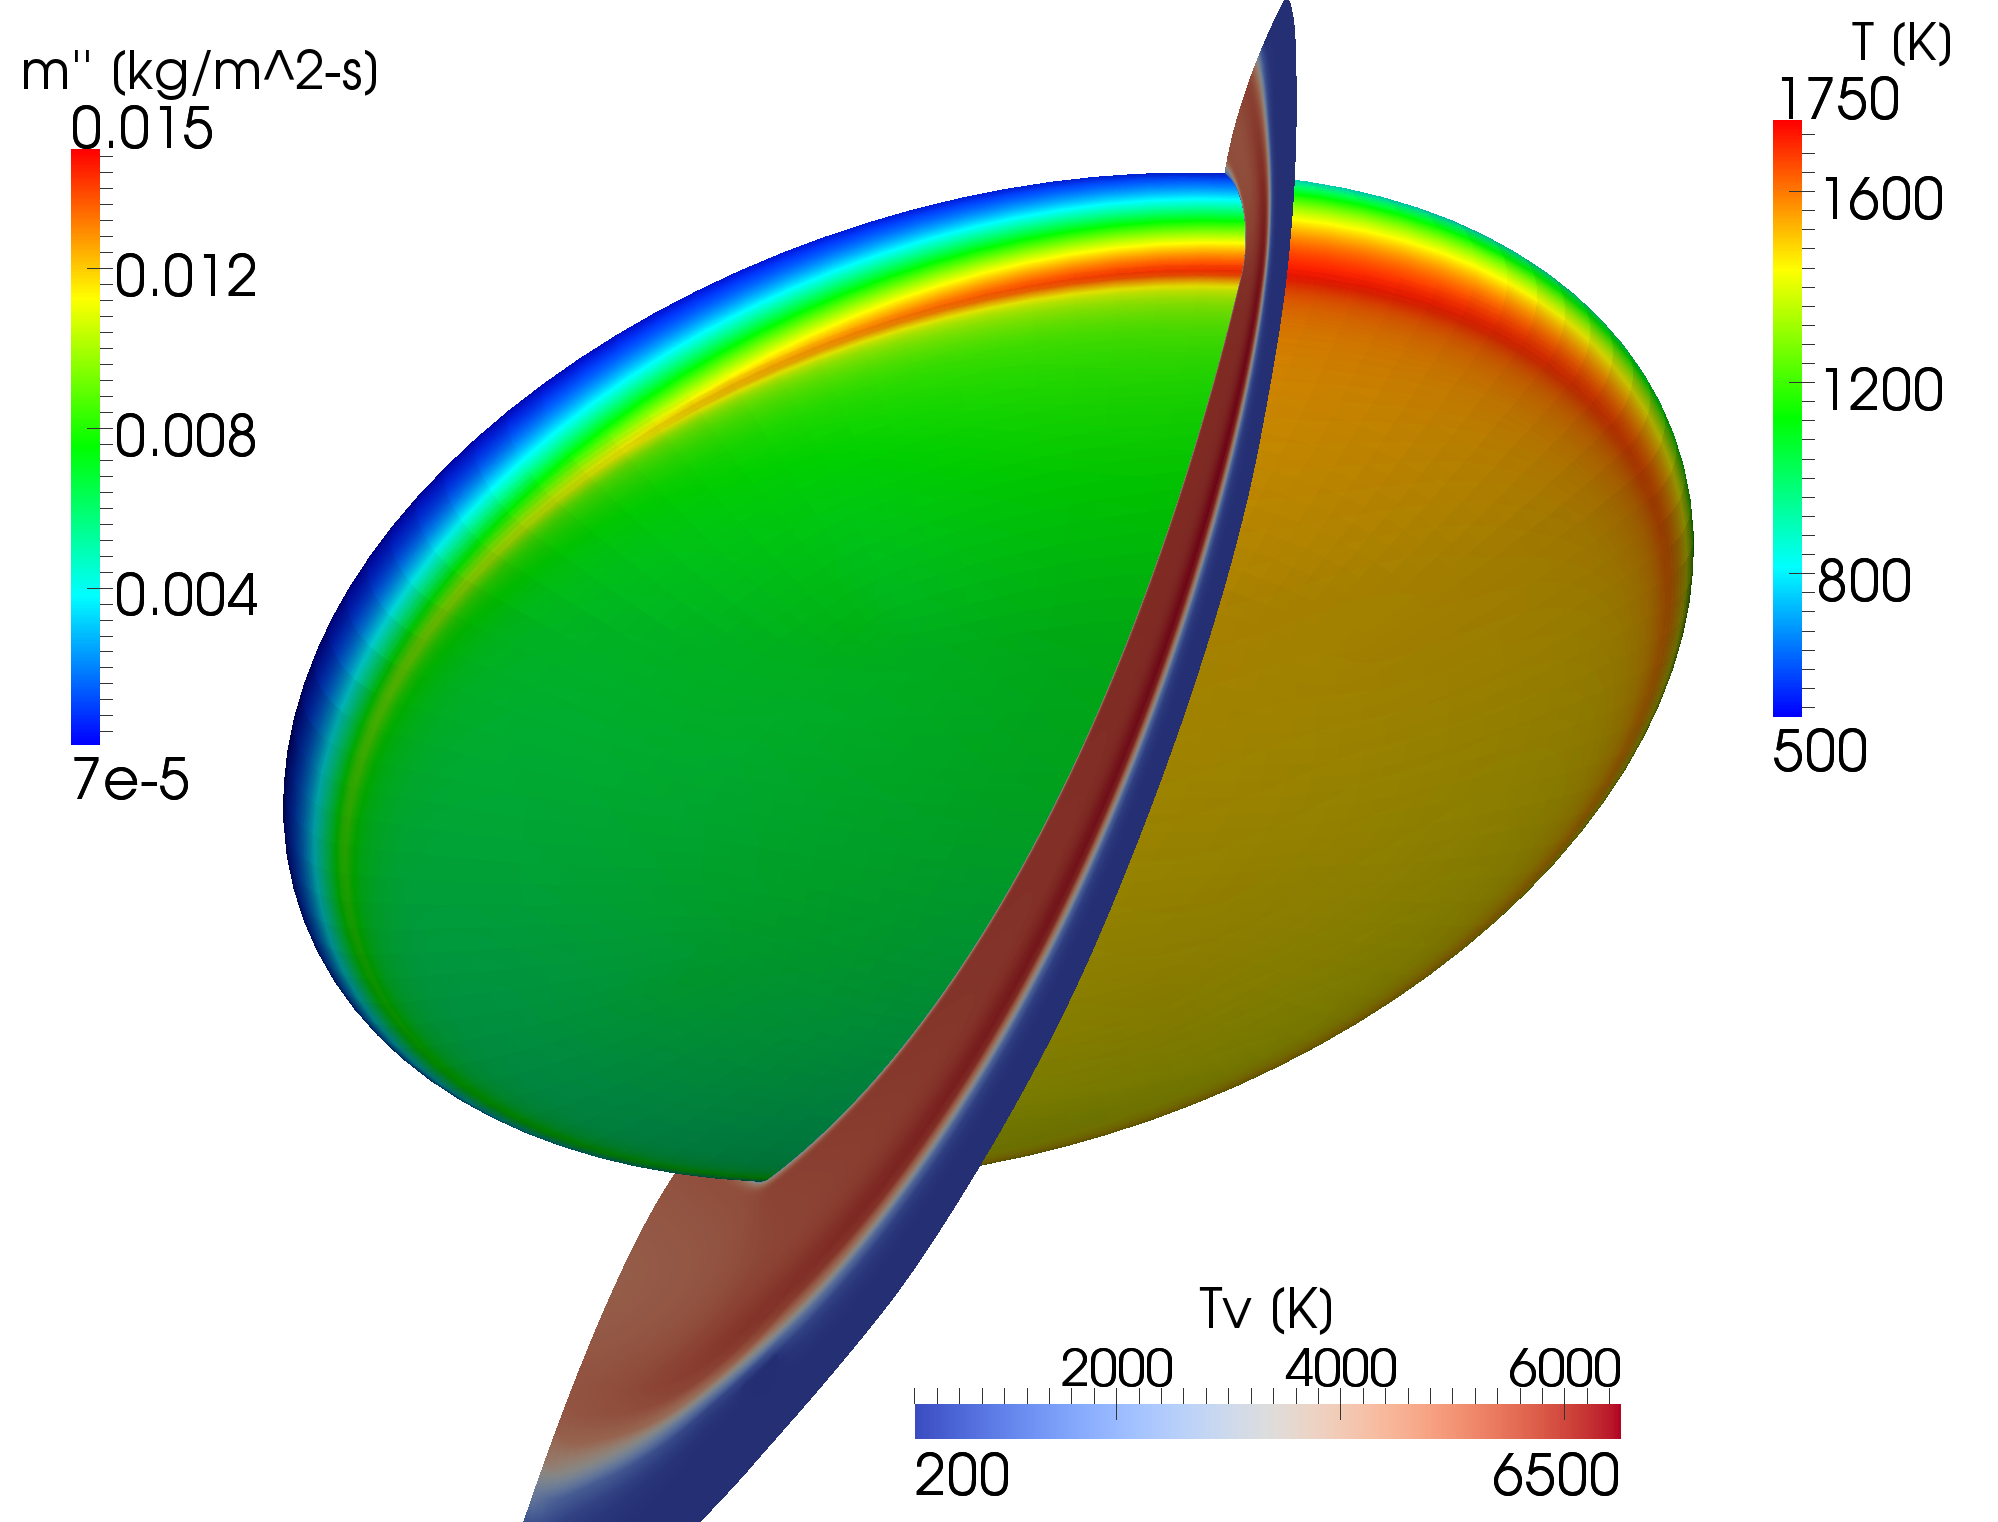
\includegraphics[height=\linewidth]{ablating_hs_wbg}}
      \end{center}
    \end{column}
  \end{columns}
}


%===============================================================================
% New Slide
%===============================================================================
\begin{frame}
\frametitle{\texttt{GRINS}}

\begin{block}{\url{https://github.com/grinsfem/grins}}
  \begin{itemize}
  \item Multiphysics FEM platform built on \texttt{libMesh}
  \item Modular structure for ``Physics'', solvers, QoIs, etc.
  \item Key feature: automatically enabled discrete adjoints (AMR, sensitivities)
  \end{itemize}
\end{block}

\begin{columns}[T]
  \begin{column}{0.4\textwidth}
    \uncover<2->{\centerline{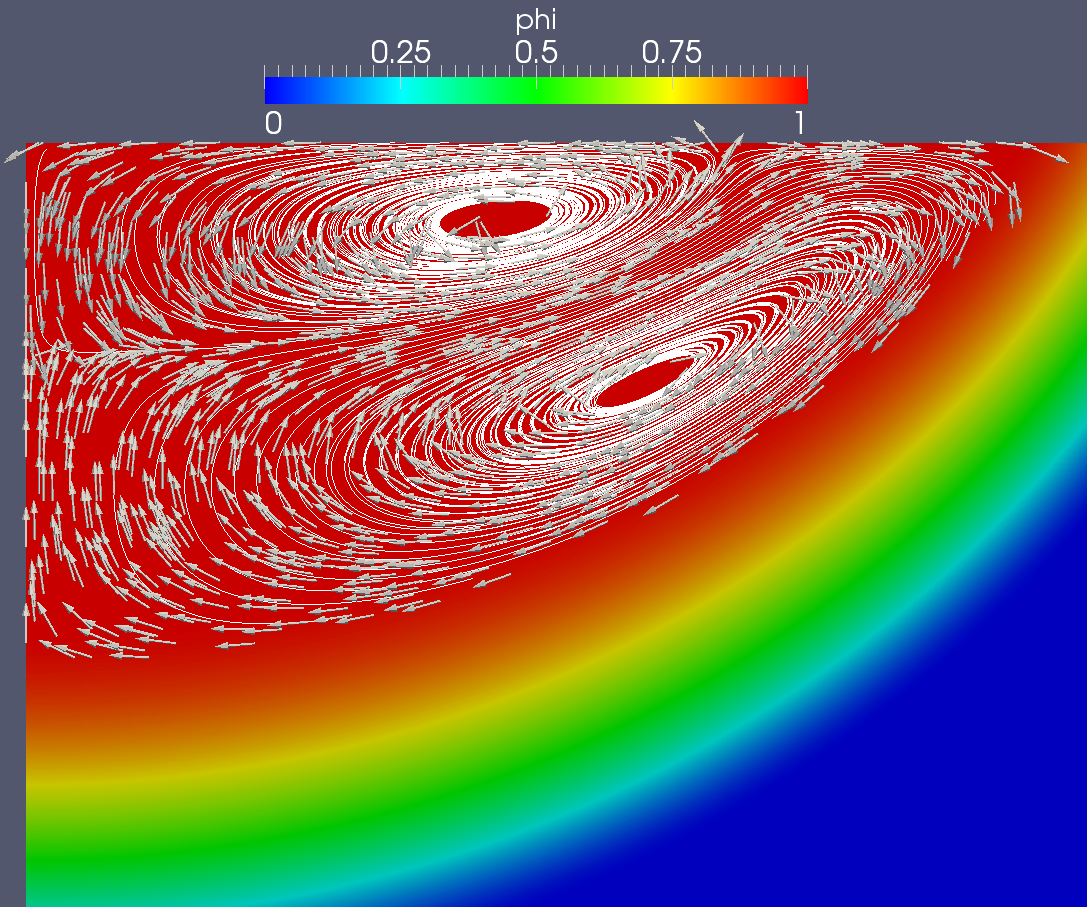
\includegraphics[width=\linewidth]{var_vortices}}}
  \end{column}
  %
  \begin{column}{0.4\textwidth}
    \only<3>{\centerline{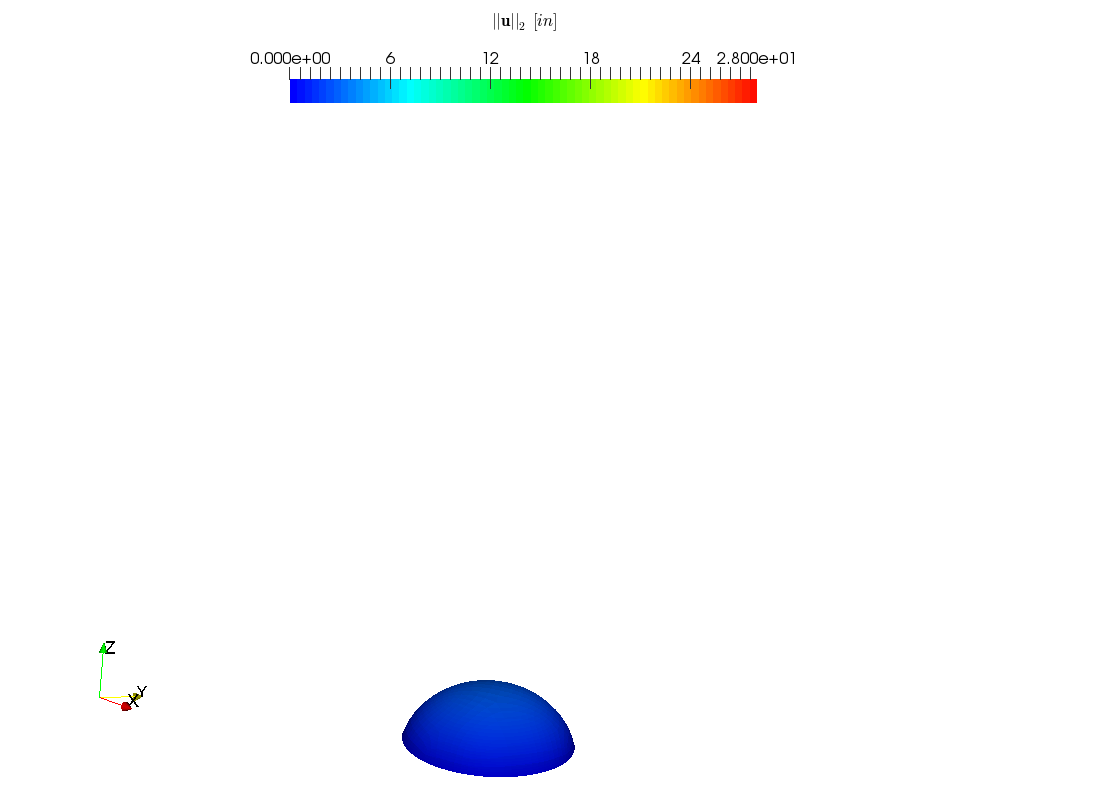
\includegraphics[width=\linewidth]{balloon_1}}}
    \uncover<4->{\centerline{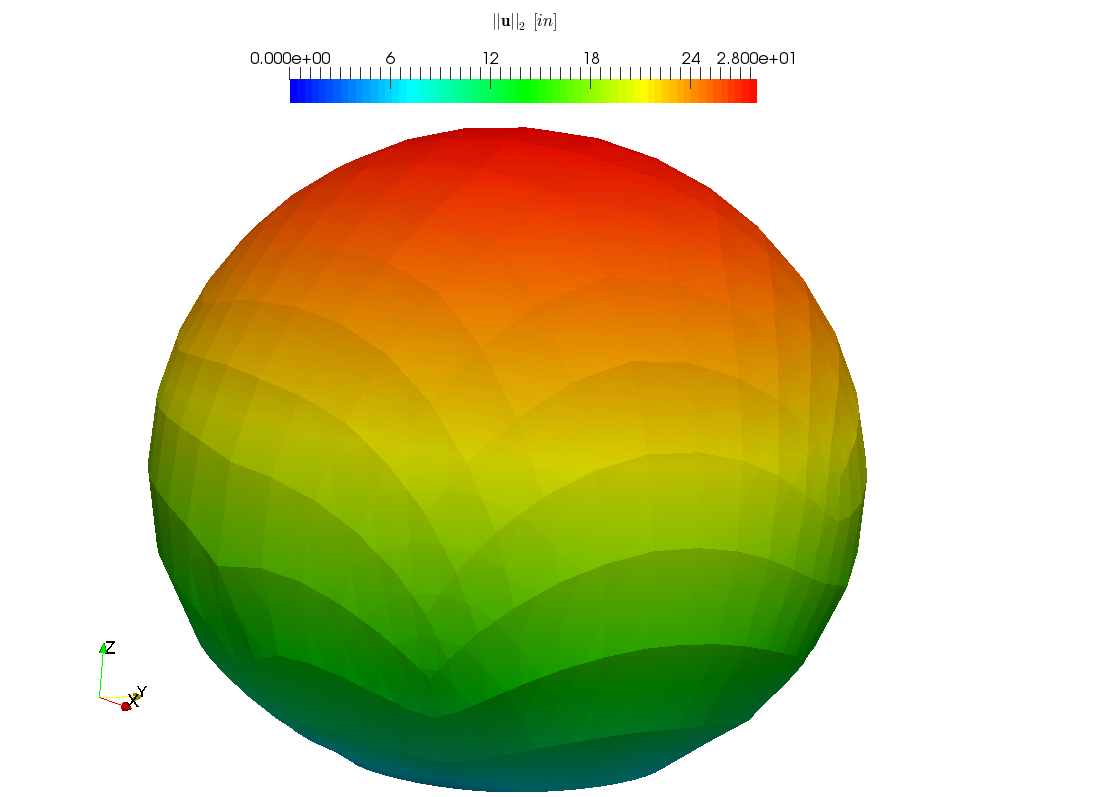
\includegraphics[width=\linewidth]{balloon_4}}}
  \end{column}
  %
  \begin{column}{0.2\textwidth}
    \uncover<5->{\centerline{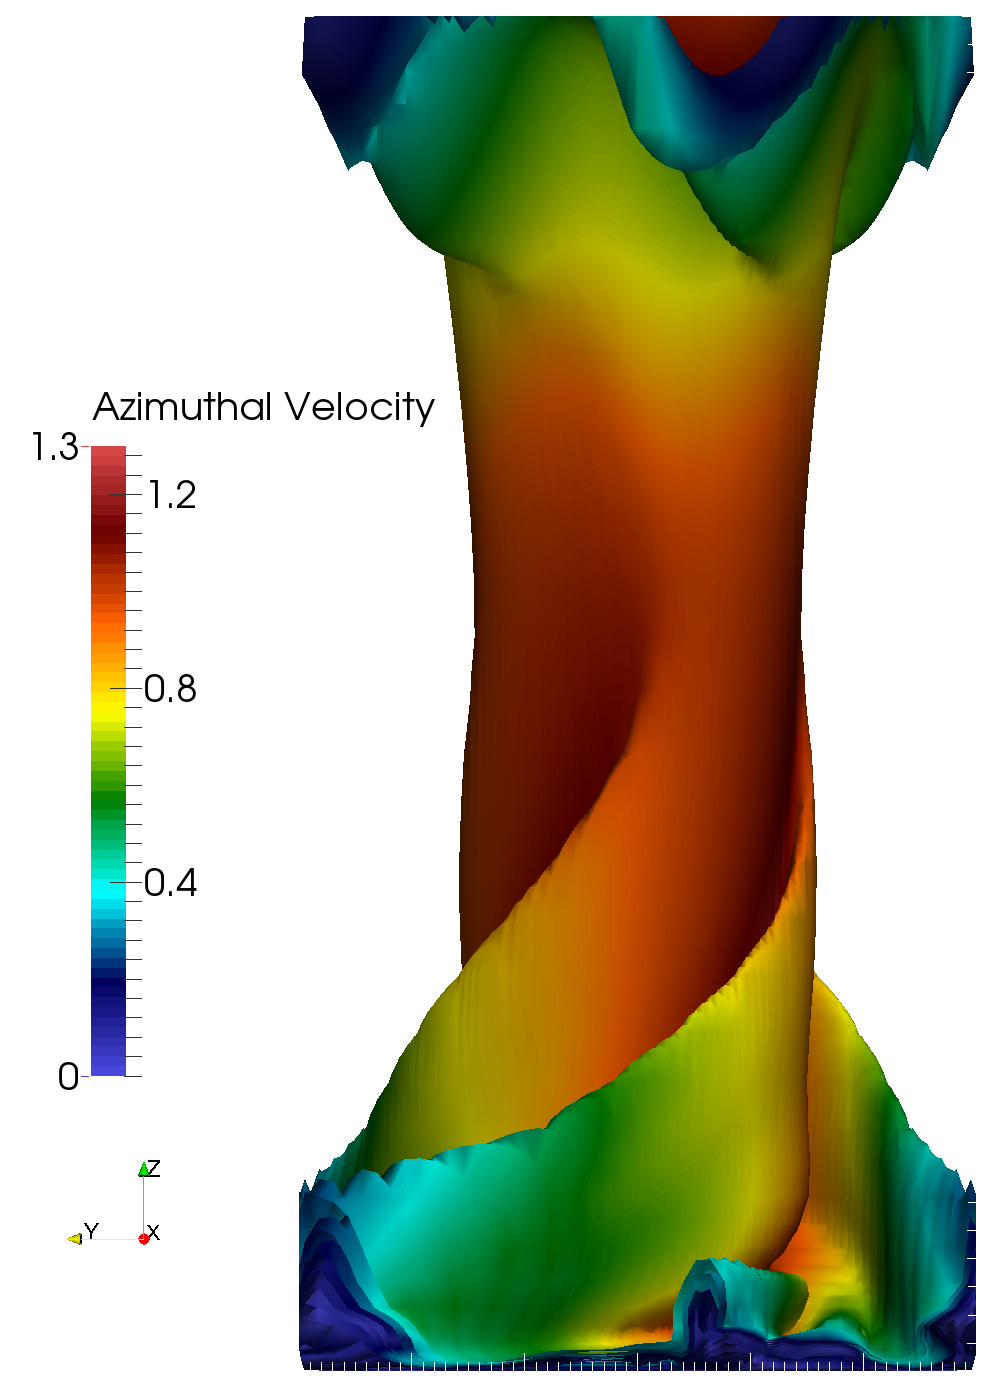
\includegraphics[width=\linewidth]{sov}}
    \tiny{Courtesy Nick Malaya, UT Austin}}
  \end{column}
  \end{columns}

\end{frame}



\frame
{
  \frametitle{The MOOSE Framework - Gaston et al., INL}
  \begin{center}
    \fbox{\includegraphics[page=2,height=0.8\textheight]{Gaston/talk}}
  \end{center}
}



%% \frame
%% {
%%   \frametitle{The MOOSE Framework - Gaston et al., INL}
%%   \begin{center}
%%     \fbox{\includegraphics[page=4,height=0.8\textheight]{Gaston/talk}}
%%   \end{center}
%% }



\frame
{
  \frametitle{The MOOSE Framework - Gaston et al., INL}
  \begin{center}
    \fbox{\includegraphics[page=22,height=0.8\textheight]{Gaston/talk}}
  \end{center}
}

\frame
{
  \frametitle{Coupled Thermal/Solid Mechanics}
  \begin{center}

    \only<1>{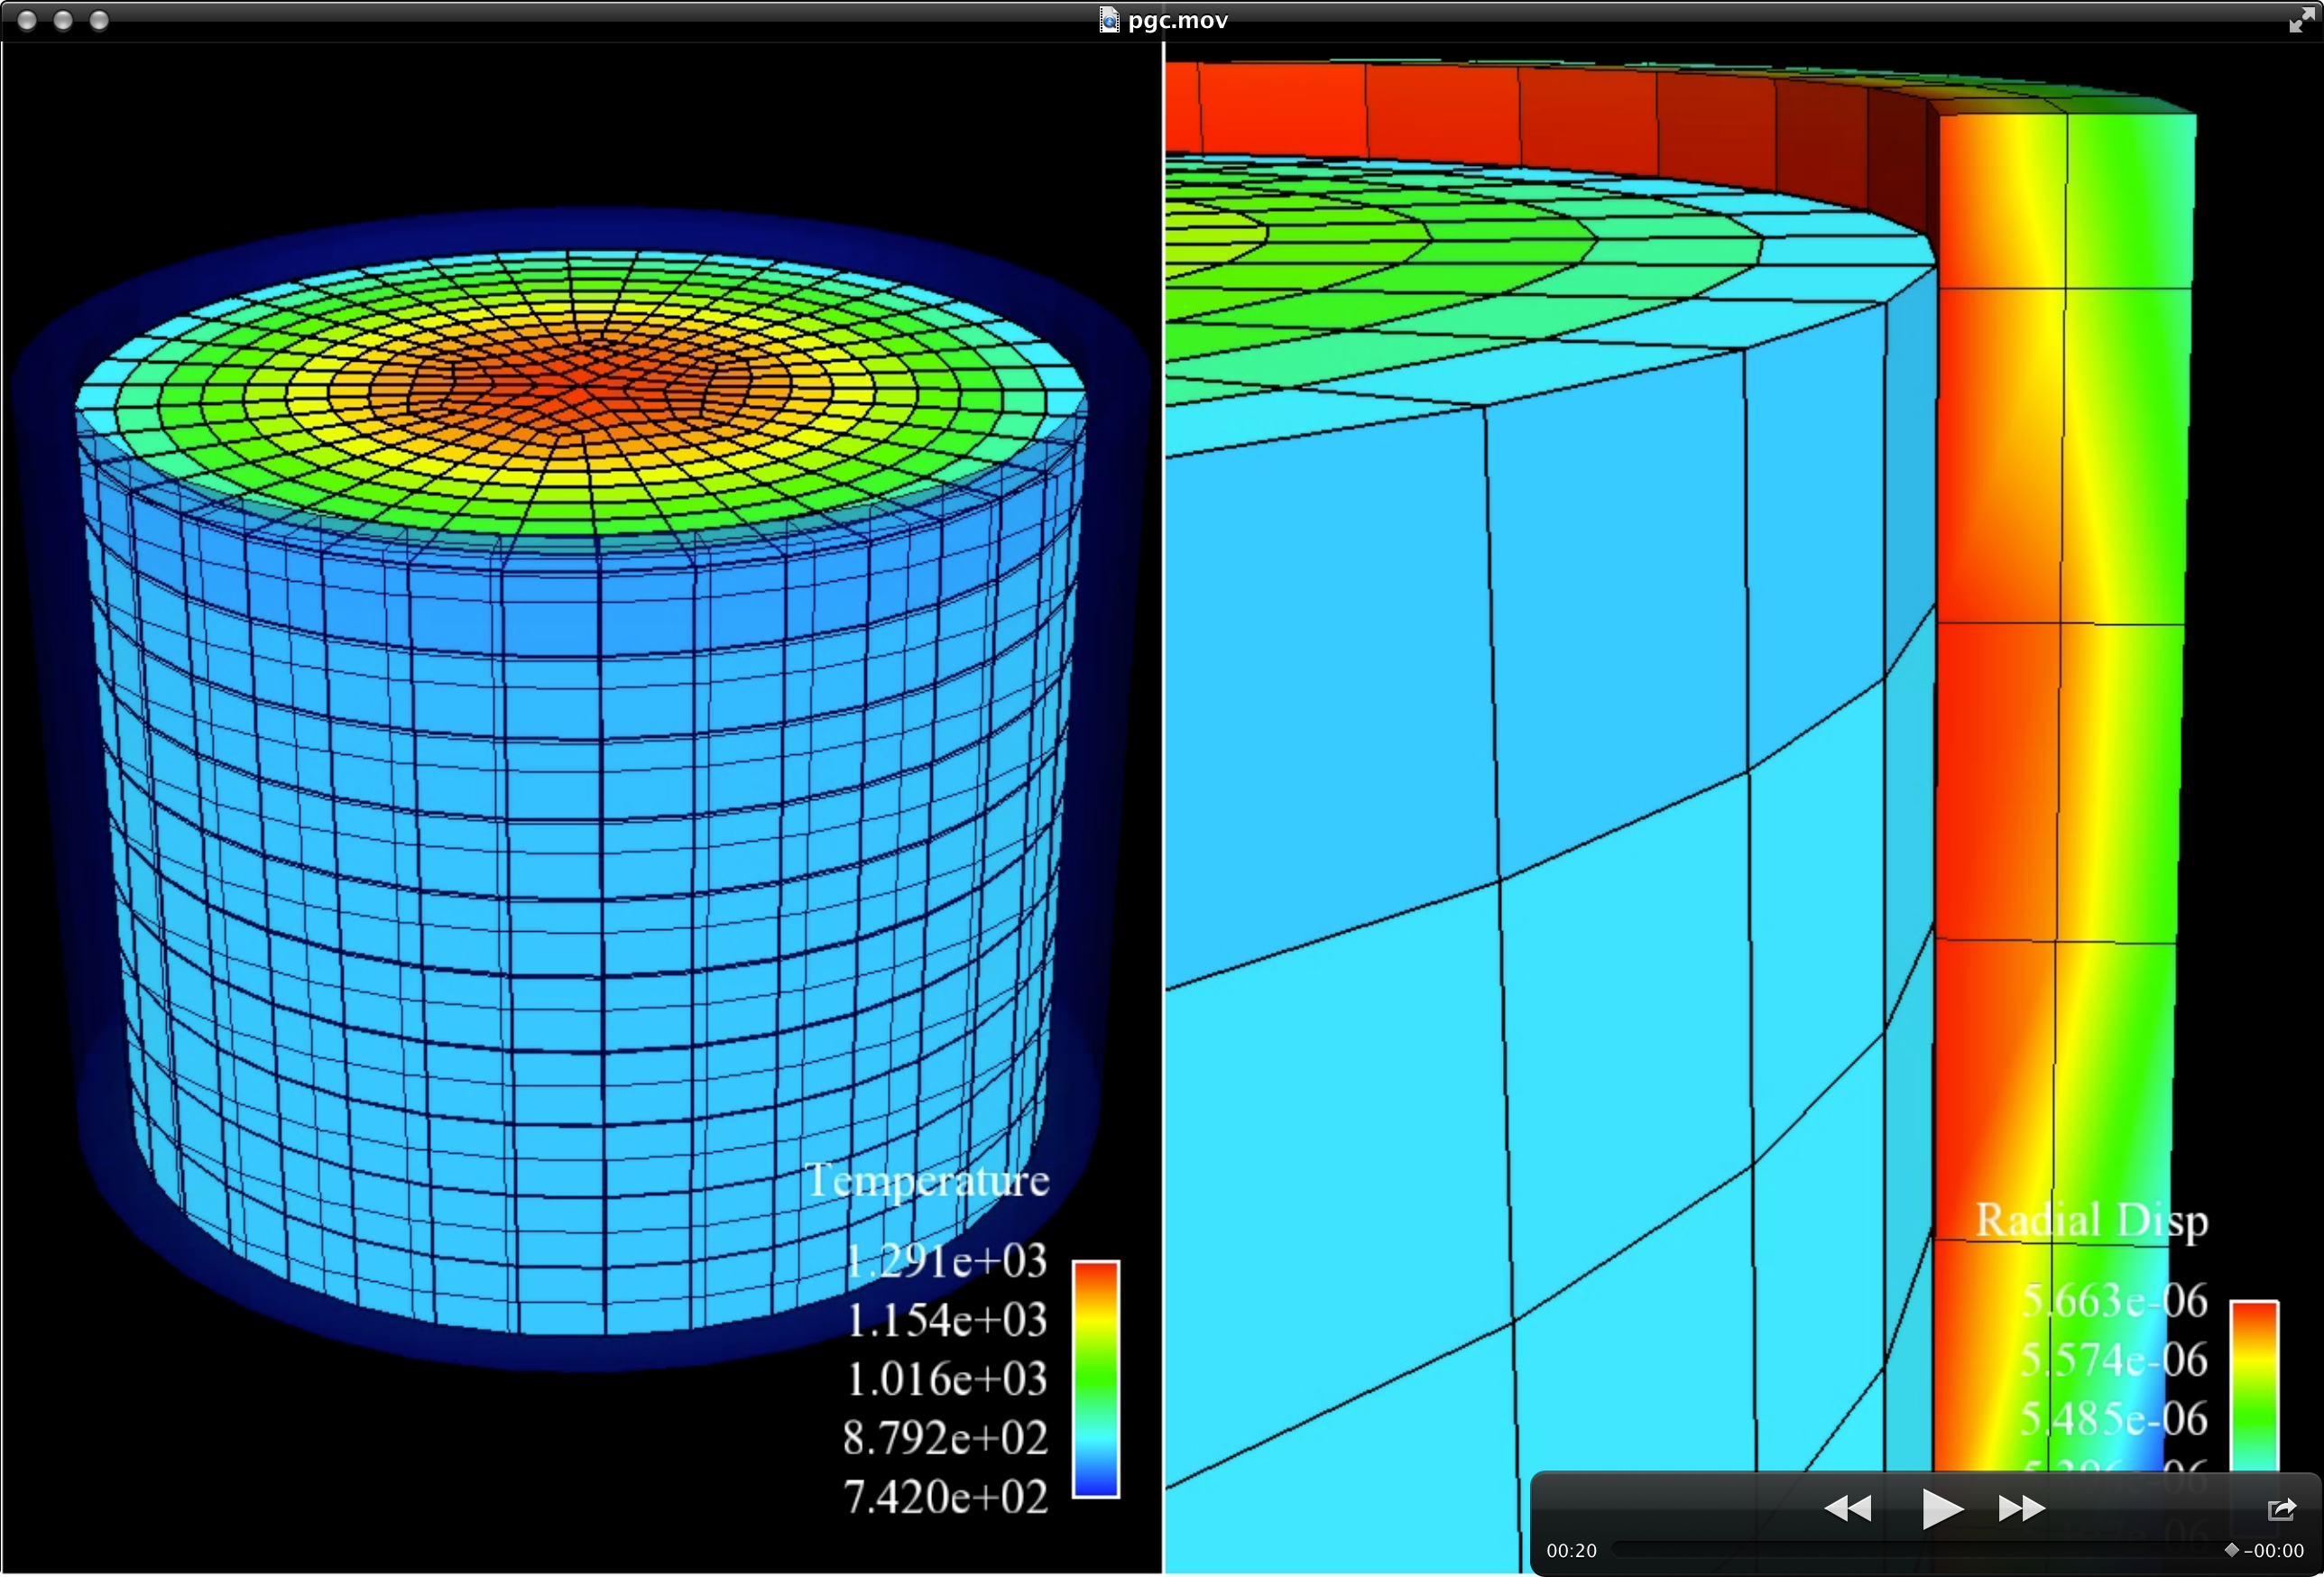
\includegraphics[height=.85\textheight]{Gaston/pgc.png}}

    \only<2>{\includemovie[autoplay,loop,text={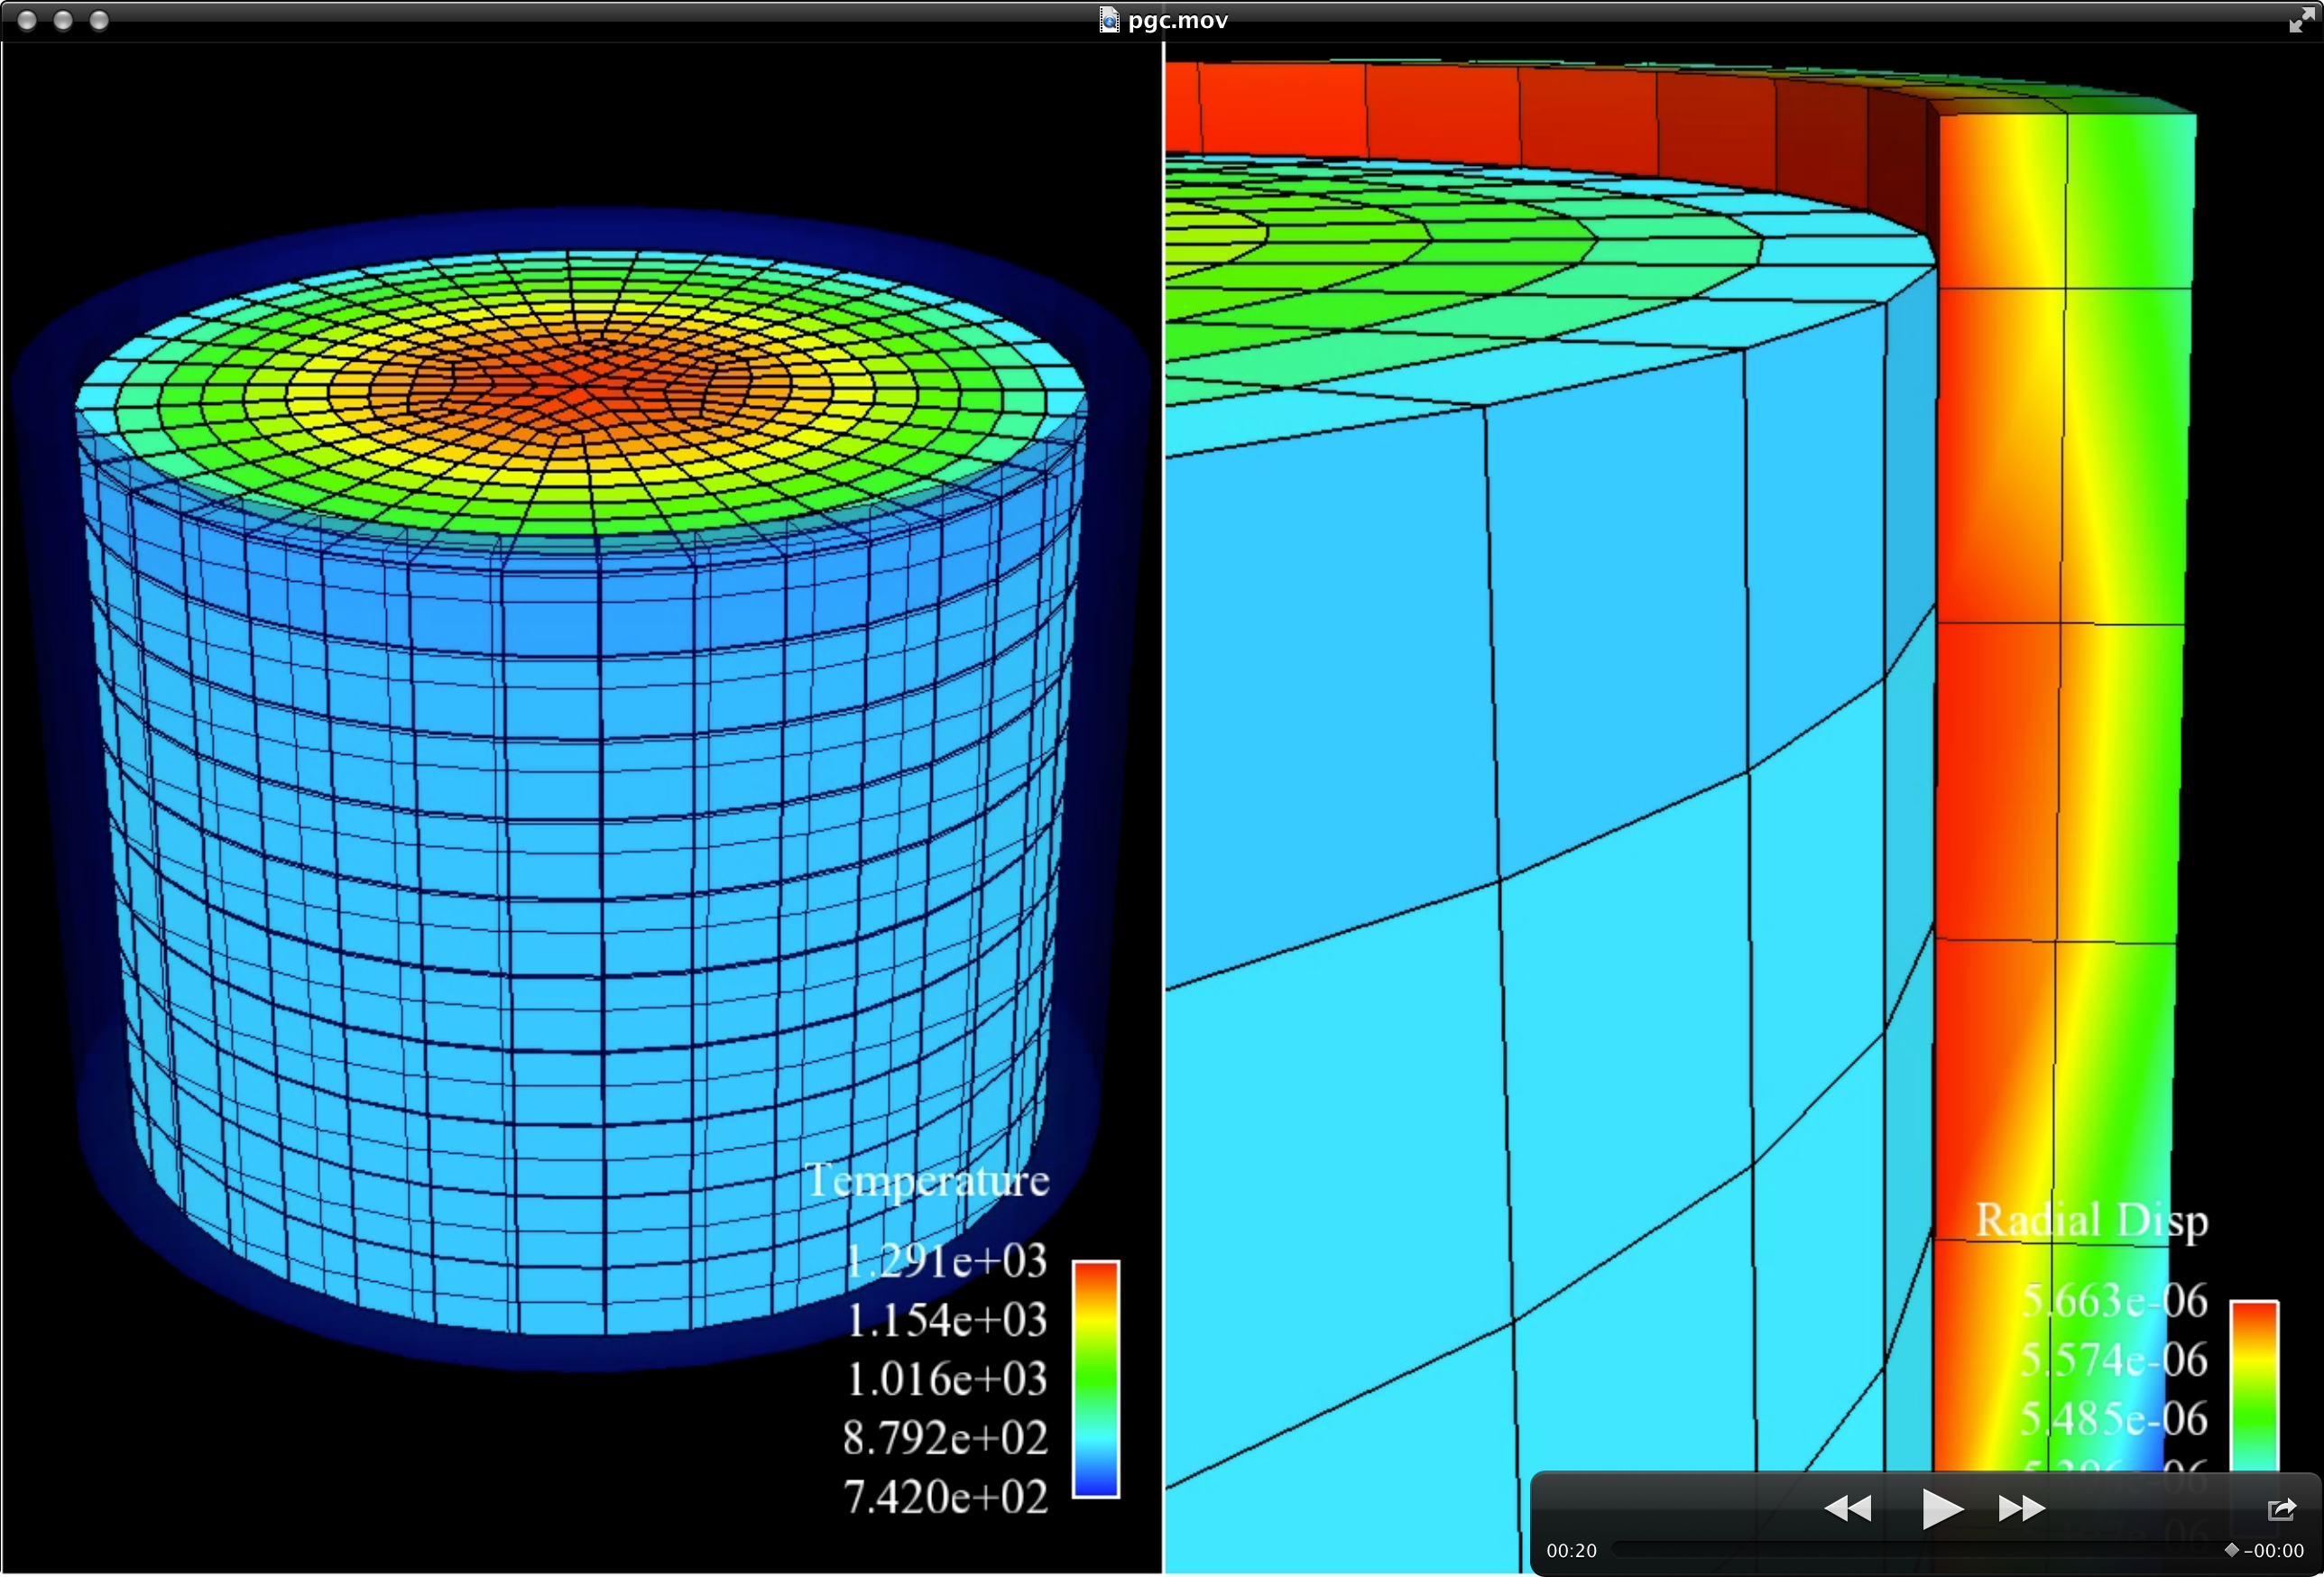
\includegraphics[height=.85\textheight]{Gaston/pgc.png}}]{}{.85\textheight}{Gaston/pgc.avi}}

  \end{center}
}

\section{Software Installation \& Ecosystem}
\subsection{Important Websites}
%%%%%%%%%%%%%%%%%%%%%%%%%%%%%%%%%%%%%%%%%%%%%%%%%
\frame
{
  \Large
  \begin{block}{}
    \center{\bf Important Websites}
    \begin{itemize}
      \item \href{http://libmesh.github.io}{Primary website}
      \item \href{http://github.com/libMesh/libmesh}{Revision Control \& Collaboration with GitHub}
      \item \href{http://buildbot.ices.utexas.edu:8010/waterfall}{Continuous Integration with Buildbot}
        %% \begin{itemize}
        %%   \item \href{http://buildbot.ices.utexas.edu:8010/builders/libmesh\%2Fmaster}{Vanilla Master}
        %%   \item \href{http://buildbot.ices.utexas.edu:8010/builders/libmesh\%2Fmaster%2Bsl6options}{Options}
        %% \end{itemize}
    \end{itemize}
  \end{block}
}


\frame
{
\frametitle{\url{http://libmesh.github.io}}

\centerline{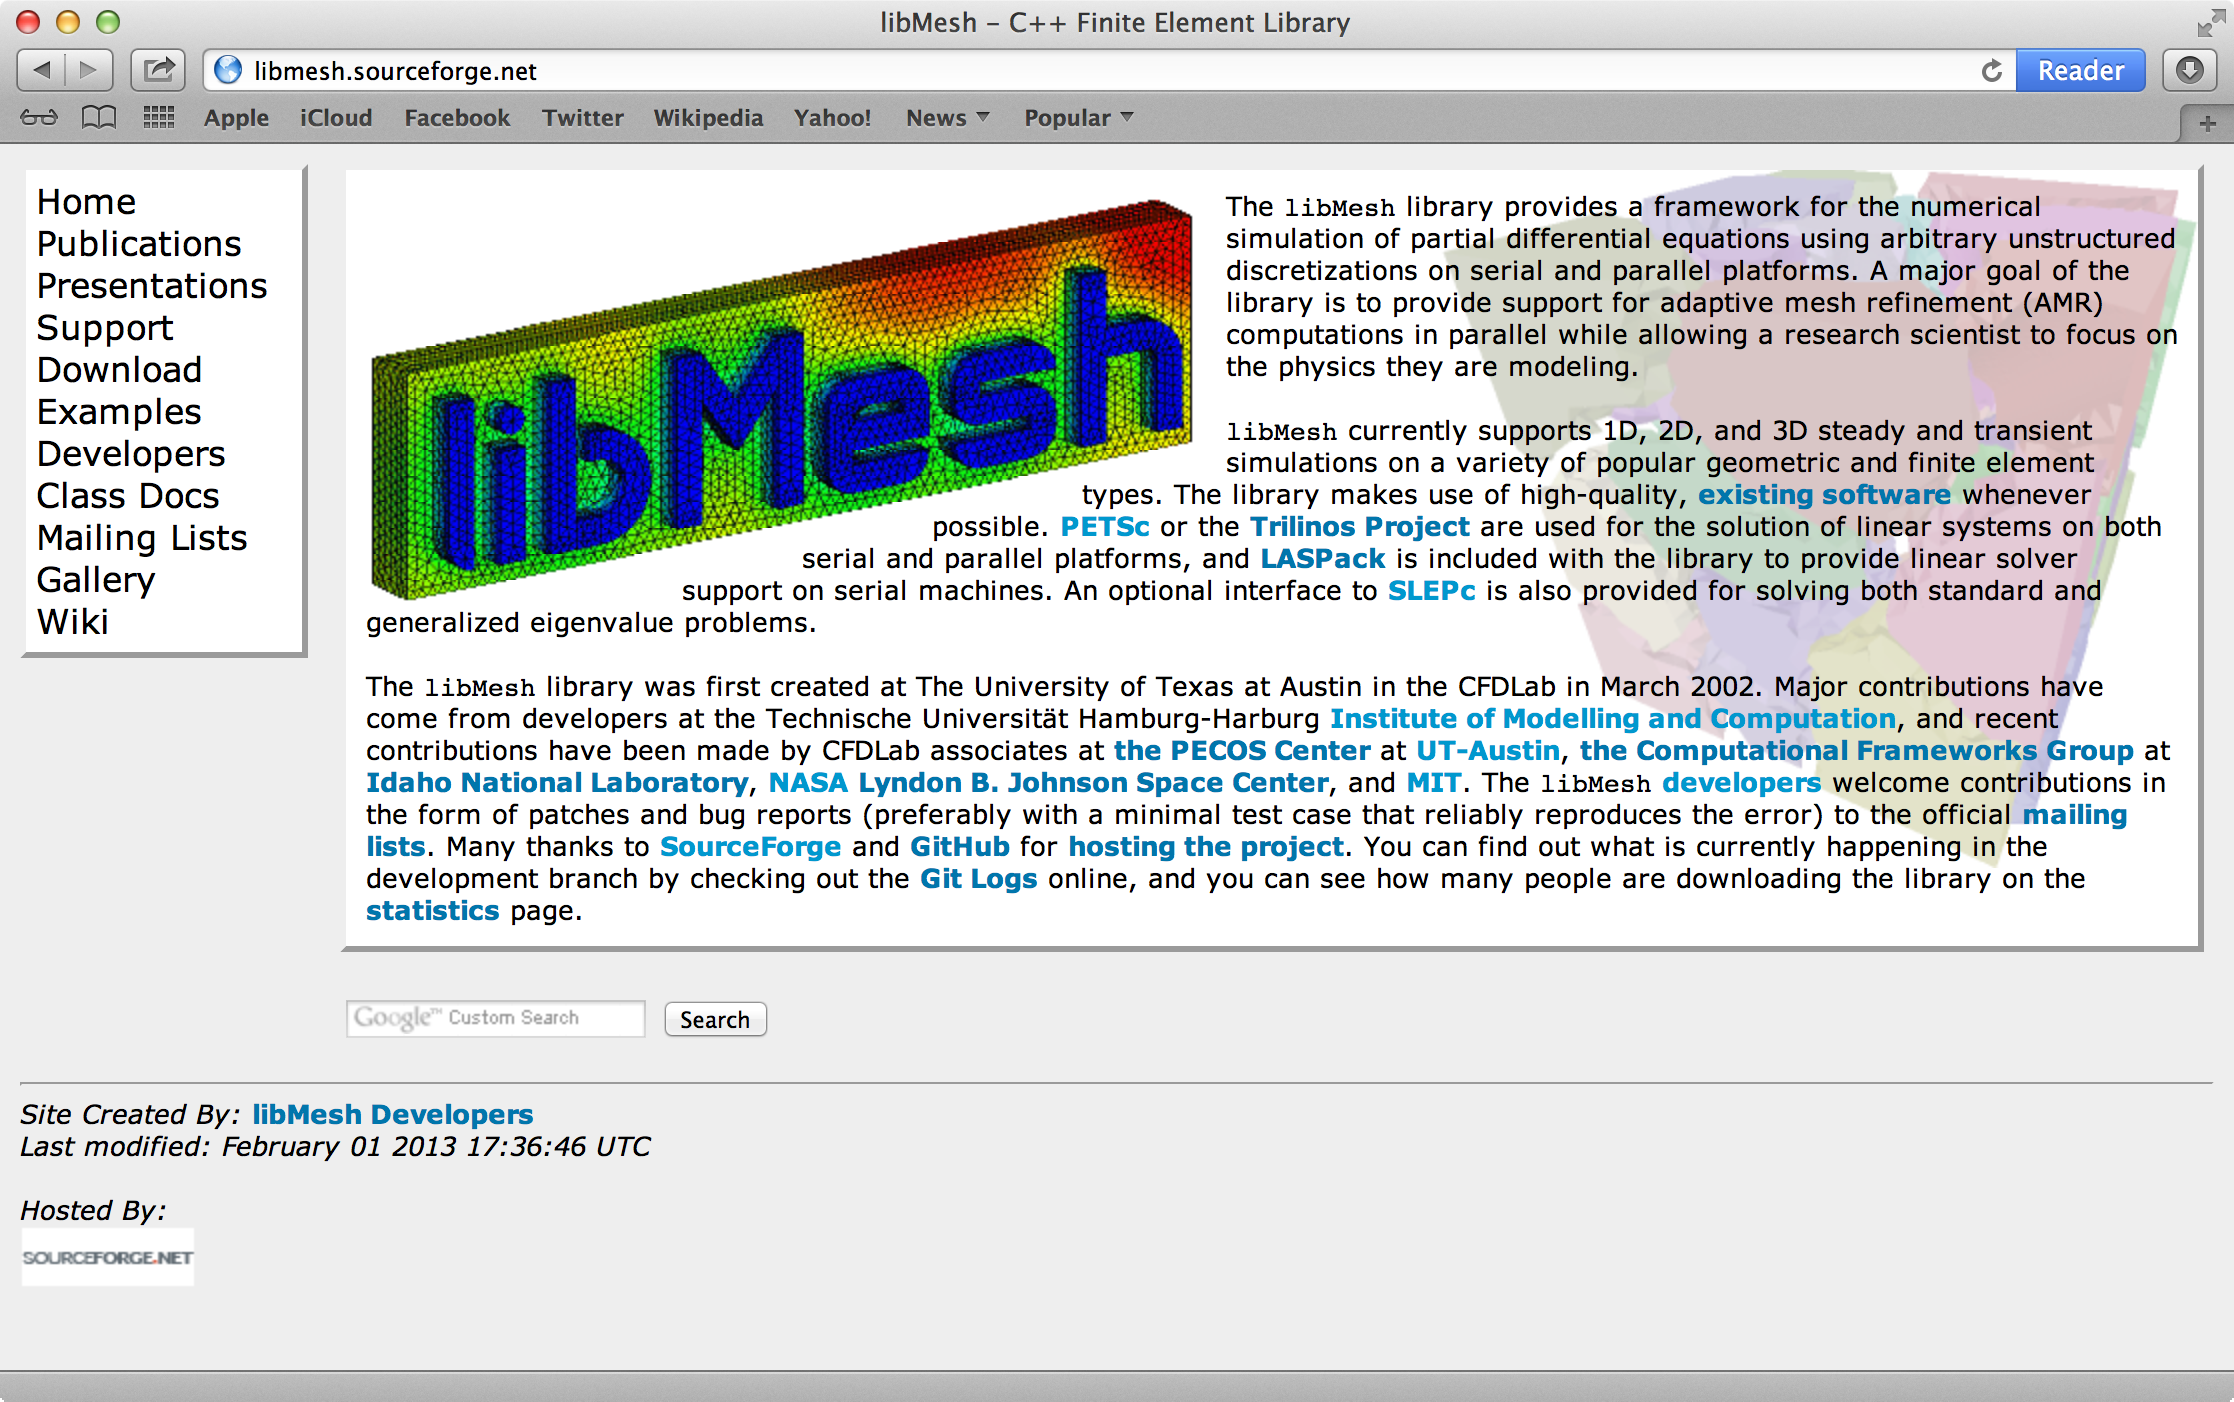
\includegraphics[height=0.85\textheight]{trivia/libmesh_site}}
}


\frame
{
\frametitle{\url{http://github.com/libMesh/libmesh}}

\centerline{\includegraphics[width=0.85\textwidth]{trivia/github_site}}
}


\frame
{
\frametitle{\scriptsize \url{http://buildbot.ices.utexas.edu:8010/waterfall}}

\centerline{\includegraphics[width=0.85\textwidth]{trivia/buildbot_site}}
}



\subsection{Compiling the library}
\frame
{
  \Large
  \begin{block}{}
    \center{\bf Building \libMesh{}}
  \end{block}
}


\begin{frame}[fragile]
  \frametitle{Getting the \libMesh{} Source}

  \begin{block}{}
    \begin{itemize}
    \item \textbf{Blessed, Stable releases:}

      Download prepackaged releases from

      \scriptsize{\url{http://github.com/libMesh/libmesh/releases}}
      \normalsize
    \item \textbf{Development tree:}

      Grab the latest source tree from GitHub:
      \begin{lstlisting}[language=bash]
$ git clone git://github.com/libMesh/libmesh.git
      \end{lstlisting}
    \end{itemize}
  \end{block}
\end{frame}

\begin{frame}
  \frametitle{\libMesh{} Suggested Dependencies}
  \begin{itemize}
    \item  \texttt{MPI} is of course required for shared-memory parallelism.
    \item Out of the box, \libMesh{} will build with support for serial linear systems.
    \item Highly recommended you first install \texttt{PETSc} and/or \texttt{Trilinos}, which \libMesh{} uses for solving linear systems in parallel.
      \item Other recommended, optional packages are:
        \begin{itemize}
          \item \texttt{SLEPc}: eigenvalue support on top of \texttt{PETSc}.
          \item Intel's Threading Building Blocks for shared-memory multithreading.
        \end{itemize}
  \end{itemize}
\end{frame}

\begin{frame}[fragile]
  \frametitle{Building \libMesh{} from source}

  \begin{block}{Unpack, Configure, Build, Install, \& Test}
    \begin{lstlisting}[language=bash]
# unpack the distribution
$ tar jxf libmesh-0.9.4-rc1.tar.bz2 && cd libmesh-0.9.4-rc1
# configure, install into the current directory
$ ./configure --prefix=$PWD/install
# build & install
$ make -j 4 && make -j 4 install
# run all the examples, but only the optimized flavor
$ make -j 4 check METHODS=opt
    \end{lstlisting}
  \end{block}
\end{frame}



\begin{frame}[fragile]
  \frametitle{Building \libMesh{} from source}

  \begin{block}{Advanced Configurations}
    \begin{lstlisting}[language=bash]
# unpack the distribution
$ tar jxf libmesh-0.9.4-rc1.tar.bz2 && cd libmesh-0.9.4-rc1
# build in a subdirectory, allows multiple simultaneous builds
$ mkdir -p clang && cd clang
# configure specifing optional packages & compilers
$ ../configure --prefix=$PWD/install \
               --with-glpk-include=/opt/local/include \
               --with-glpk-lib=/opt/local/lib \
               --with-vtk-include=/opt/local/include/vtk-5.10 \
               --with-vtk-lib=/opt/local/lib/vtk-5.10 \
               --with-eigen-include=/opt/local/include/eigen3 \
               --with-cxx=clang++-mp-3.3 --with-cc=clang-mp-3.3 \
               --disable-fortran
# build & install
$ make -j 4 && make -j 4 install
    \end{lstlisting}
  \end{block}
\end{frame}



\begin{frame}[fragile,shrink]
  \frametitle{Building \libMesh{} from source}

  \begin{block}{Testing the Installation}
    \begin{lstlisting}[language=bash]
$ make -j 4 installcheck
Making installcheck in include
Making installcheck in libmesh

Checking for standalone headers in installed tree ...

Testing Header libmesh/libmesh_config.h ...            [   OK   ]
Testing Header base/auto_ptr.h ...                     [   OK   ]
Testing Header base/dirichlet_boundaries.h ...         [   OK   ]
Testing Header base/dof_map.h ...                      [   OK   ]
Testing Header base/dof_object.h ...                   [   OK   ]
...

Checking for self-sufficient examples...

Testing examples in /tmp/libmesh-0.9.4-rc1/_inst/examples
Testing example installation adaptivity/ex1 ...        [   OK   ]
Testing example installation adaptivity/ex2 ...        [   OK   ]
Testing example installation adaptivity/ex3 ...        [   OK   ]
Testing example installation adaptivity/ex4 ...        [   OK   ]
Testing example installation adaptivity/ex5 ...        [   OK   ]
...
    \end{lstlisting}
  \end{block}
\end{frame}



\subsection{Compiling Applications}
\frame
{
  \Large
  \begin{block}{}
    \center{\bf Getting Started with \libMesh{} Applications}
  \end{block}
}



\begin{frame}[fragile,shrink]
  \frametitle{The \libMesh{} installation}

  \begin{block}{Installation Tree}
    \begin{lstlisting}[language=bash]
# henceforth we assume LIBMESH_DIR points to the installation path
$ cd $LIBMESH_DIR
$ ls
Make.common contrib     examples    lib
bin         etc         include     share
$ ls lib | grep mesh
libmesh_dbg.0.dylib
libmesh_dbg.dylib
libmesh_dbg.la
libmesh_devel.0.dylib
libmesh_devel.dylib
libmesh_devel.la
libmesh_opt.0.dylib
libmesh_opt.dylib
libmesh_opt.la
$ ls lib/pkgconfig
Make.common      libmesh-devel.pc libmesh-opt.pc   libmesh.pc
libmesh-dbg.pc   libmesh-oprof.pc libmesh-prof.pc  netcdf.pc
    \end{lstlisting}
  \end{block}
\end{frame}



\begin{frame}[fragile,shrink]
  \frametitle{The \libMesh{} installation}

  \begin{block}{Compiling Simple Applications with \texttt{pkg-config}}
    \begin{lstlisting}[language=bash]
# make sure pkg-config can find the libMesh configuration
$ export PKG_CONFIG_PATH=$LIBMESH_DIR/lib/pkgconfig:$PKG_CONFIG_PATH

# copy the first example program
$ cp -r $LIBMESH_DIR/examples/introduction/ex1 . && cd ex1

# see what we've got
$ ls
Makefile introduction_ex1.C run.sh

# compile against the full debug version of libMesh
$ mpicxx -o introduction_ex1 introduction_ex1.C \
  `pkg-config --cflags --libs libmesh-dbg`

# compile against the default, optimized version of libMesh
$ mpicxx -o introduction_ex1 introduction_ex1.C \
  `pkg-config --cflags --libs libmesh`
    \end{lstlisting}
  \end{block}
\end{frame}






\begin{frame}[fragile,shrink]
  \frametitle{The \libMesh{} installation}

  \begin{block}{Compiling Simple Applications with \texttt{libmesh-config}}
    \begin{lstlisting}[language=bash]
# we support a similar utility, libmesh-config, which predates
# pkg-config support. this is similar, but also can report the
# compiler used.
$ PATH=$LIBMESH_DIR/bin:$PATH

$ libmesh-config
usage: libmesh-config --cppflags --cxxflags --include --libs
       libmesh-config --cxx
       libmesh-config --cc
       libmesh-config --fc
       libmesh-config --fflags
       libmesh-config --version
       libmesh-config --host

# get the name of the compiler used, as passed to ./configure
$ libmesh-config --cxx
mpicxx
    \end{lstlisting}
  \end{block}
\end{frame}



\begin{frame}[fragile,shrink]
  \frametitle{The \libMesh{} installation}

  \begin{block}{Compiling Applications with \texttt{make}}
    \begin{lstlisting}[language=bash]
# copy the first example program
$ cp -r $LIBMESH_DIR/examples/introduction/ex1 . && cd ex1

# compile against the default, optimized version of libMesh
$ make
Compiling C++ (in optimized mode) introduction_ex1.C...
Linking example-opt...

# compile against the full debug version of libMesh
$ make METHOD=dbg
Compiling C++ (in debug mode) introduction_ex1.C...
Linking example-dbg...
    \end{lstlisting}
  \end{block}
\end{frame}



\begin{frame}[fragile,shrink]
  \frametitle{A first \libMesh{} application}
  \begin{lstlisting}
#include <iostream>
#include "libmesh/libmesh.h"
#include "libmesh/mesh.h"

using namespace libMesh;

int main (int argc, char** argv)
{
  LibMeshInit init (argc, argv);

  if (argc < 4)
    {
      if (libMesh::processor_id() == 0)
        std::cerr << "Usage: " << argv[0] << " -d 2 in.mesh [-o out.mesh]"
                  << std::endl;

      libmesh_error();
    }

  Mesh mesh(init.comm());

  mesh.read (argv[3]);

  mesh.print_info();

  if (argc >= 6 && std::string("-o") == argv[4])
    mesh.write (argv[5]);

  return 0;
}
  \end{lstlisting}
\end{frame}



\begin{frame}[fragile,shrink]
  \frametitle{A first \libMesh{} application}
  \begin{lstlisting}[language=bash]
# copy & build the example
$ cp -r $LIBMESH_TUTORIAL/basic .
$ cd basic
$ make
Compiling C++ (in optimized mode) introduction_ex1.C...
Linking example-opt...

# run the example, reading a trivial mesh and writing output
$ ./example-opt -d 3 \
  $LIBMESH_DIR/share/reference_elements/3D/one_hex27.xda -o out.exo
 Mesh Information:
  mesh_dimension()=3
  spatial_dimension()=3
  n_nodes()=27
    n_local_nodes()=27
  n_elem()=1
    n_local_elem()=1
    n_active_elem()=1
  n_subdomains()=1
  n_partitions()=1
  n_processors()=1
  n_threads()=1
  processor_id()=0
  \end{lstlisting}
\end{frame}

\section{A Generic Boundary Value Problem}
%%%%%%%%%%%%%%%%%%%%%%%%%%%%%%%%%%%%%%%%%%%%%%%%%

\subsection*{A Generic BVP}

\begin{frame}[t]
  \frametitle{Typical Boundary Value Problem}
  \begin{columns}[t]
    \column{.5\textwidth}
     \begin{itemize}
      \item Common BVP components:
      \vspace{-.1in}
        \begin{eqnarray}
        \label{eqn:general_pde}
        \nonumber
        \bv{M} \frac{\partial \bv{u}}{\partial t} & = & \bv{F}( \bv{u} ) \;\, \in \Omega \subset \Reals^n
        \\
        \nonumber
        \bv{G}( \bv{u} ) & = & 0 \;\;\;\;\;\;\;\; \in \Omega
        \\
        \nonumber
        \bv{u} & = & \bv{u}_D \;\;\;\;\; \in \partial \Omega_D
        \\
        \nonumber
        \bv{N}(\bv{u}) & = & 0 \;\;\;\;\;\;\;\; \in \partial \Omega_N
        \\
        \nonumber
        \bv{u}(\bv{x}, 0) & = & u_0(\bv{x}) 
      \end{eqnarray}
      \item Less common components:
        \begin{itemize}
        \item Moving domain $\Omega(t)$, $\Omega(\bv{u},t)$
        \item Multi-dimensional manifolds
        \item Self-overlapping, contact
        \item Acceleration ${\partial^2 u}/{\partial t^2}$
        \item Integro-differential equations
        \end{itemize}
      \end{itemize}
    \column{.5\textwidth}
      \begin{center}
        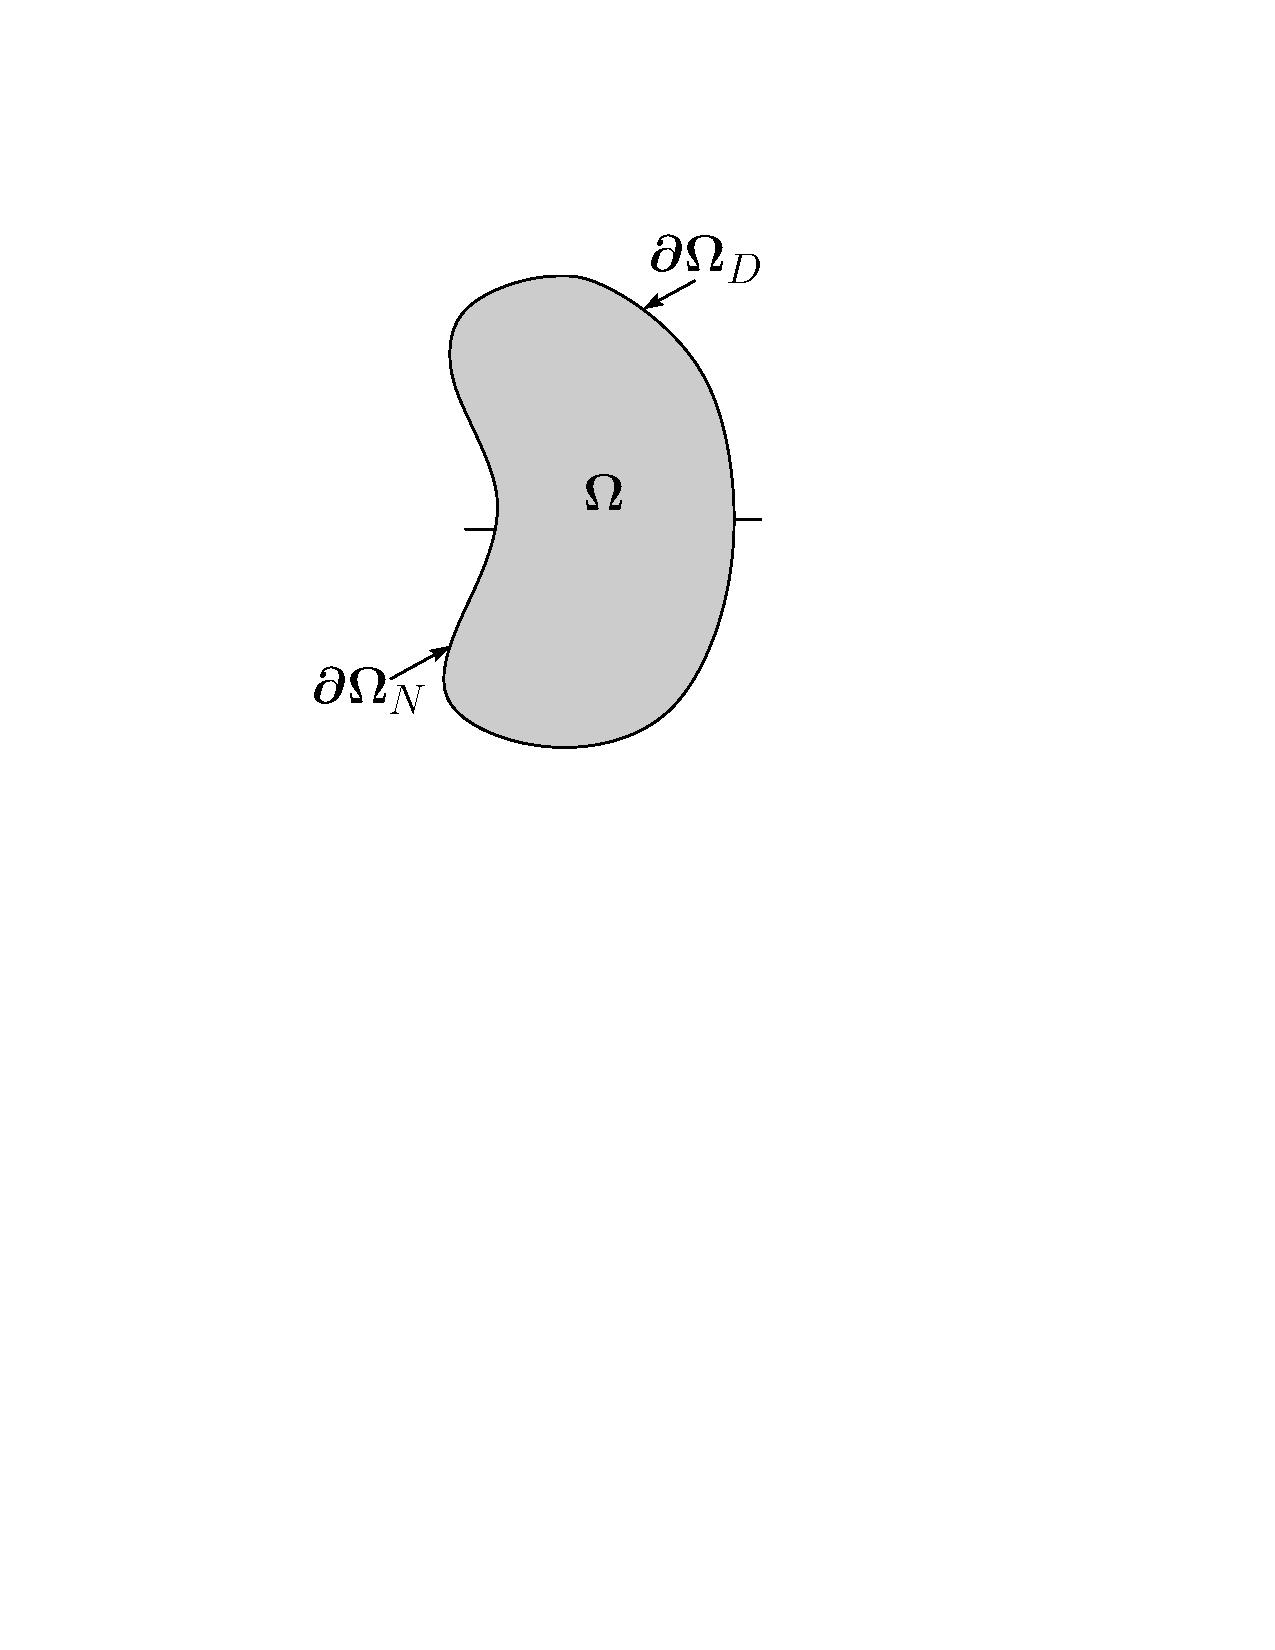
\includegraphics[viewport=140 420 400 685,clip=true,width=.5\textwidth]{domain2_input}
        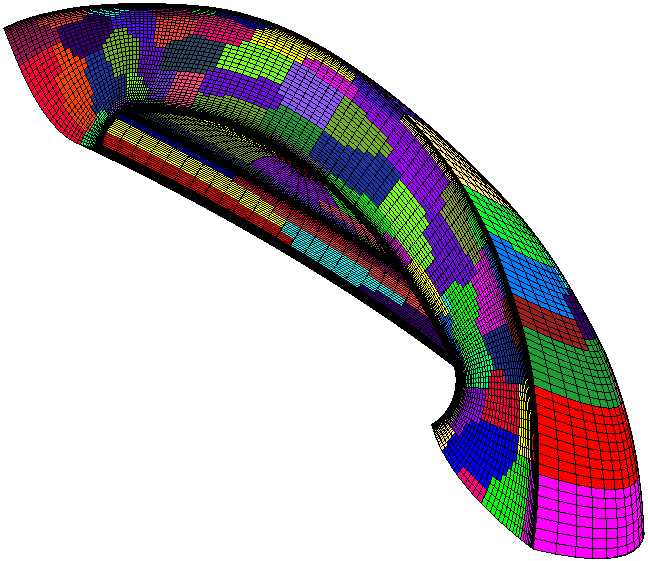
\includegraphics[width=.5\textwidth]{capsule_partitioned}

        \includegraphics[width=.45\textwidth]{fins-transition} \;
        \includegraphics[width=.45\textwidth]{sheet_perspective}

      \end{center}
  \end{columns}
\end{frame}


\begin{frame}
  %\frametitle{}
  \begin{columns}[t]
    \column{.5\textwidth}
    \begin{block}{}%A general class of PDE}
      \begin{itemize}
      \item{
	Associated to the problem domain $\Omega$ is a \libMesh{} data
	structure called a \texttt{Mesh}
      }

      \item{A \texttt{Mesh} is essentially
	a collection of finite elements}
      \end{itemize}
      \begin{equation}
	\label{eqn:discretized_domain}
	\nonumber
	\Omega^h:=\bigcup_e \Omega_e
      \end{equation}
    \end{block}
    %\pause
    \column{.5\textwidth}
    %\begin{block}{}
      \begin{center}
	%\fbox{
	\includegraphics[width=2in,angle=-90]{discretized_domain}
	%}
      \end{center}
    %\end{block}
  \end{columns}
  \visible<2>
  {
  \begin{itemize}
    \item{\libMesh{} provides some simple structured mesh generation
routines, interfaces to Triangle and TetGen, and supports a rich set of input file formats.}
  \end{itemize}
  }
\end{frame}


\section{Key Data Structures}

%%%%%%%%%%%%%%%%%%%%%%%%%%%%%%%%%%%%%
\subsection{The Mesh Class}

\begin{frame}
  \frametitle{Operations on Objects in the \texttt{Mesh}}
  \begin{block}{}
    \begin{itemize}
    \item From a \texttt{Mesh} it is trivial to access ranges of objects of interest through \emph{iterators}.
    \item Iterators are simply a mechanism for accessing a range of objects.
    \item \libMesh{} makes extensive use of \emph{predictated iterators} to access, for example,
      \begin{itemize}
        \item All elements in the mesh.
        \item The ``active'' elements in the mesh assigned to the local processor in a parallel simulation.
        \item The nodes in the mesh.
      \end{itemize}
  \end{itemize}
  \end{block}
\end{frame}

\begin{frame}[shrink]
  \frametitle{Mesh Iterators}
  \lstinputlisting{snippets/active_elem_iterators.cxx}
\end{frame}

\begin{frame}[shrink]
  \frametitle{Mesh Iterators}
  \lstinputlisting{snippets/node_iterators.cxx}
\end{frame}



%%%%%%%%%%%%%%%%%%%%%%%%%%%%%%%%%%%%%
\subsection{The EquationSystems Class}
\begin{frame}
  \frametitle{EquationSystems}
  \begin{block}{}
    \begin{itemize}
      \item The \texttt{Mesh} is a discrete representation of the geometry for a problem.
      \item For a given \texttt{Mesh}, there can be an \texttt{EquationSystems} object, which represents one or more coupled system of equations posed on the \texttt{Mesh}.
        \begin{itemize}
          \item There is only one \texttt{EquationSystems} object per \texttt{Mesh} object.
          \item The \texttt{EquationSystems} object can hold many \texttt{System} objects, each representing a logical system of equations.
        \end{itemize}
      \item High-level operations such as solution input/output is usually handled at the \texttt{EquationSystems} level.
    \end{itemize}
  \end{block}
\end{frame}

\begin{frame}[shrink]
  \frametitle{EquationSystems}
  \lstinputlisting{snippets/es.cxx}
\end{frame}




%%%%%%%%%%%%%%%%%%%%%%%%%%%%%%%%%%%%%
\subsection{The Elem Class}
\begin{frame}
  \frametitle{Elements}
  \begin{block}{}
    \begin{itemize}
      \item The \texttt{Elem} base class defines a geometric element in \libMesh{}.
      \item An \texttt{Elem} is defined by \texttt{Node}s, Edges (2D,3D) and Faces (3D).
      \item An \texttt{Elem} is sufficiently rich that in many cases it is the only argument required to provide to a function.
    \end{itemize}
  \end{block}
\end{frame}

\begin{frame}[shrink]
  \frametitle{Elements}
  \lstinputlisting{snippets/elem.cxx}
\end{frame}

 

%%%%%%%%%%%%%%%%%%%%%%%%%%%%%%%%%%%%%
\subsection{The \texttt{Node} Class}
\begin{frame}
  \frametitle{Nodes}
  \begin{block}{}
    \begin{itemize}
      \item \texttt{Node}s define spatial locations in arbitrary dimensions.
      \item Logically, a \texttt{Node} is a point in \emph{N}-space plus metadata:
        \begin{itemize}
          \item Global ID.
          \item Processor ownership.
          \item Degree of freedom indexing data.
        \end{itemize}
    \end{itemize}
  \end{block}
\end{frame}

\begin{frame}
  \frametitle{Nodes}
  \lstinputlisting{snippets/node.cxx}
\end{frame}


\section{Weighted Residuals}
%% Auto-generate the TOC slide(s)
\begin{frame}
  \tableofcontents[currentsection]
  %\tableofcontents
\end{frame}


\begin{frame}[<+->]
      %\frametitle{Weighted Residual Statement}
  \begin{itemize}
  \item {The point of departure in any FE analysis which uses \libMesh{} is
    the weighted residual statement
    %(sometimes referred to as simply ``the residual'' in
    %the documentation.)
    \begin{equation}
      \nonumber
      (F( u ), v) = 0 \hspace{.5in} \forall v \in \mathcal{V}
    \end{equation}
    }

  \item{ Or, more precisely, the weighted residual statement associated with the
    finite-dimensional space $\mathcal{V}^h \subset \mathcal{V}$
    \begin{equation}
      \nonumber
      (F( u^{\alert{h}} ), v^{\alert{h}}) = 0 \hspace{.5in} \forall v^{\alert{h}} \in \mathcal{V}^{\alert{h}}
  \end{equation}}

  \item{ Even stabilized formulations boil down to some semilinear
          form
    \begin{equation}
      \nonumber
      \Res( u^{\alert{h}}, v^{\alert{h}}) = 0 \hspace{.5in} \forall v^{\alert{h}} \in \mathcal{V}^{\alert{h}}
  \end{equation}}

  \end{itemize}
\end{frame}


\subsection*{Some Examples}    
\begin{frame}[t]
  %\frametitle{Some Examples}
    \begin{block}{
	\only<1-2>{Poisson Equation}
	\only<3-4>{Linear Convection-Diffusion}
	\only<5-6>{Stokes Flow}
      }

      \only<1-2>
      {
	\begin{equation}
	      \nonumber
	      -\Delta u  = f
	      \hspace{.25in} \in \hspace{.1in} \Omega  
	    \end{equation}
      }
      
      \only<3-4>
	  {
	    \begin{equation}
	      \nonumber
	      %\frac{\partial u}{\partial t}
	      -k\Delta u + \bv{b} \cdot \nabla u = f
	      \hspace{.25in} \in \hspace{.1in} \Omega  
	    \end{equation}
	  }

      \only<5-6>
      {
	\begin{equation}
	    \begin{array}{rcl}
	      \nonumber
	      %\frac{\partial \bv{u}}{\partial t} +
	      %\left(\bv{u} \cdot \nabla\right) \bv{u} +
	      \nabla p - \nu \Delta \bv{u}  &=& \bv{f}
	        \\
	      \nonumber
	      \nabla \cdot \bv{u} &=& 0
	    \end{array}  \hspace{.25in}  \in \hspace{.1in} \Omega
	\end{equation}
      }

      
\end{block}
    %\pause

    \only<2,4,6>
    {
    \begin{block}{Weighted Residual Statement}
    }
      \only<2>
      {
      \begin{eqnarray}
	\nonumber
	(F( u ), v) := %\hspace{3in} \\  \nonumber
	\int_{\Omega}  \left[ \nabla u \cdot \nabla v - fv \right] dx \\ \nonumber
	+ \int_{\partial \Omega_N} \left(\nabla u \cdot \bv{n}\right) v \;ds
      \end{eqnarray}
%%       $^{\ast}$ We have employed the divergence theorem to obtain the weighted residual statement.
%%       In general this procedure gives rise to boundary terms which for simplicity we do not discuss
%%       in detail.
      }
      
    \only<4>
    {
      \begin{eqnarray}
	\nonumber
	(F( u ), v) := 
	\int_{\Omega} \left[
	  %\tfrac{\partial u}{\partial t}v  +
	  k\nabla u \cdot \nabla v + (\bv{b} \cdot \nabla u) v - fv \right] dx \\ \nonumber
	+ \int_{\partial \Omega_N} k\left(\nabla u \cdot \bv{n}\right) v \;ds
      \end{eqnarray}
    }

    \only<6>
    {
      \vspace{-.2in}
      \begin{eqnarray}
	\nonumber
	u := \left[\bv{u}, p\right]
	\hspace{.1in},\hspace{.1in}
	v := \left[\bv{v}, q\right]
      \end{eqnarray}
      \vspace{-.25in}
	\begin{eqnarray}
	  \nonumber
	(F( u ), v) := %\hspace{3in} \\ \nonumber
	\int_{\Omega} \left[
	  %\left( \tfrac{\partial \bv{u}}{\partial t}	  +
	  %\left( \bv{u} \cdot \nabla  \right)\bv{u}
	  %\right)
	  %\cdot \bv{v}
	- p\left(\nabla \cdot \bv{v}\right) 
	+ \nu \nabla \bv{u} \colon\!\! \nabla \bv{v} - \bv{f}\cdot \bv{v} \; \right. \\ \nonumber
	+ \left.\left( \nabla \cdot \bv{u} \right) q \right] dx
	+ \int_{\partial \Omega_N} \left(\nu \nabla \bv{u} -p\bv{I}\right)  \bv{n} \cdot \bv{v} \;ds %\hspace{1in}	
      \end{eqnarray}
    }
\only<2,4,6>
{
    \end{block}
 }     
\end{frame} 



%\subsection*{Approximate Problem}
\begin{frame}%[<+->]
  %\frametitle{Weighted Residual Statement}
  \begin{itemize}

    %%   \item{In each of the examples, the weighted residual statement is obtained by
    %%     multiplying the PDE by a test function $v$, integrating over the domain $\Omega$,
    %%     and applying the divergence theorem.}

    %%   \item{Since $v=0$ on $\partial \Omega_D$ (essential data) the boundary integrals
    %%     are over $\partial \Omega_N$ only.}

    %%   \item{There are simple and efficient techniques (e.g.\ penalty method) for
    %%     enforcing the Dirichlet conditions.}

  \item{To obtain the approximate problem, we simply
    replace $u \leftarrow u^h$, $v \leftarrow v^h$, and $\Omega \leftarrow \Omega^h$
    in the weighted residual
    statement.}
    
  \end{itemize}
\end{frame}

\subsection{Poisson Equation}
%% Auto-generate the TOC slide(s)
\begin{frame}
  \tableofcontents[currentsection]
  %\tableofcontents
\end{frame}


\subsection*{Weighted Residual Statement}
\begin{frame}%[<+->]
  %\frametitle{Poisson Equation}
  \begin{itemize}
  \item {For simplicity we start with the weighted
    residual statement arising from the Poisson equation,
    with $\partial \Omega_N = \emptyset$, 
    \begin{eqnarray}
      \nonumber
      (F( u^h ), v^h) := \hspace{2.5in} \\  \nonumber
      \int_{\Omega^h}  \left[ \nabla u^h \cdot \nabla v^h - fv^h \right] dx %\\ \nonumber
      %+ \int_{\partial \Omega^h_N} u_N v^h \;ds
      =0 \hspace{.5in} \forall v^{h} \in \mathcal{V}^{h}
    \end{eqnarray}
  }
  \end{itemize}
\end{frame}

\subsection*{Element Integrals}
\begin{frame}%[c]
%  \frametitle{Poisson Equation}
  \begin{itemize}    
  \item{
%%     \only<1>
%% 	{
	  The integral over $\Omega^h$ \ldots
%%	}
	  \visible<2->
	  {
	    is written as
	    a sum of integrals over the $\alert{N_e}$ finite elements: % $\Omega_e^h$
	  }
  }
  \end{itemize}
	  
  %\begin{block}{}
    \begin{eqnarray}
	\nonumber
	%(F( u^h ), v^h) &:=& %\hspace{3in} \\  \nonumber
	0 &=&
	\phantom{\sum_{e=1}^{N_e}}
	\int_{\Omega^h}  \left[ \nabla u^h \cdot \nabla v^h - fv^h \right] dx
	\hspace{.2in} \forall v^{h} \in \mathcal{V}^{h}
	\\ \nonumber
	\visible<2>
	    {
	&=&\alert{\sum_{e=1}^{N_e}}
	      \int_{\alert{\Omega_e}}
	      \left[ \nabla u^h \cdot \nabla v^h - fv^h \right] dx
	      \hspace{.2in} \forall v^{h} \in \mathcal{V}^{h}
	      \\ \nonumber
	    }
%% 	    \visible<3>
%% 		{
%% 	&=&\alert{\sum_{e=1}^{N_e}}
%% 	      \underbrace{\int_{\alert{\Omega_e}}
%% 	      \left[ \nabla u^h \cdot \nabla v^h - fv^h \right] dx}_{\text{We must compute this}}
%% 	      \hspace{.2in} \forall v^{h} \in \mathcal{V}^{h}
%% 		}
      \end{eqnarray}
    %\end{block}
%%     \begin{eqnarray}
%%       \nonumber
%%       (F( u^h ), v^h) &=& \int_{\Omega^h} (\ldots) \\
%%       \nonumber
%%       &=& \sum_{e=1}^{N_e} \int_{\Omega_e}(\ldots)\hspace{.25in} \forall v^{h} \in \mathcal{V}^{h}
%%     \end{eqnarray}
    
%  \item{The $v^h$ typically have support over only a small subset of the elements.}
\end{frame}

\subsection*{Finite Element Basis Functions}
\begin{frame}
  % \frametitle{Weighted Residual Statement}
    \begin{columns}[t]
    \column{.5\textwidth}
    \begin{block}{}
%%       \only<1>
%%       {
%% 	To node $i$ we associate a basis function $\psi_i$ such that for any $v^h \in \mathcal{V}^h$
%% 	we have
%% 	\begin{equation}
%% 	  \nonumber
%% 	  v^h = \sum_{i=1}^{N_n} c_i \psi_i
%% 	\end{equation}
%% 	for some constants $c_i$.
%%       }

%%       \only<2>
%%       {
%% 	\begin{itemize}
%% 	  \item{The $\psi_i$ are non-zero only over the elements adjacent to node $i$.}
%% 	  \item{For example, $\psi_i$ could be the linear ``hat'' function.
%% 	    %with value 1
%% 	    %at node $i$ and zero at all other nodes.
%% 	  }
%% 	\end{itemize}
%%       }

%%       \only<3->
%%       {
	\begin{itemize}
	  \item{An element integral will have contributions only
	    from the global basis functions corresponding to its nodes.}
	  \item{We call these local basis functions $\phi_i$, $0 \leq i \leq N_s$.}
	\end{itemize}
%%      }
    \end{block}

%%       \visible<3->
%%       {
	    \begin{equation}
	      \nonumber
	      \left. v^h \right|_{\Omega_e} = \sum_{i=1}^{N_s} c_i \phi_i
	    \end{equation}
%%      }
      \visible<2>
      {
	    \begin{equation}
	      \nonumber
	      \alert{\int_{\Omega_e}} v^h \;\alert{dx}
	      = \sum_{i=1}^{N_s} c_i \alert{\int_{\Omega_e}}\phi_i \;\alert{dx}
	    \end{equation}

      }
%}
%  \end{itemize}
    \column{.5\textwidth}
    %\begin{block}{}
      \begin{center}
%% 	\only<1>
%% 	    {
%% 	      \includegraphics[width=2in,angle=-90]{node_i}
%% 	    }
%% 	\only<2>
%% 	    {
%% 	      \includegraphics[width=2in,angle=-90]{phi_i}
%% 	    }
%% 	\only<3->
%% 	    {
	      \includegraphics[width=2in,angle=-90]{phi_ijk}
%%	    }
      \end{center}
    \end{columns}
\end{frame}
    
\subsection*{Element Matrix and Load Vector}
\begin{frame}%[t]
%  \frametitle{Poisson Equation}
  \begin{itemize}    
    \visible<1->
	{
	\item
	  {
	    The element integrals \ldots
	    \begin{equation}
	      \nonumber
	      \int_{\Omega_e} \left[ \nabla u^h \cdot \nabla v^h - fv^h \right] dx
	    \end{equation}
	  }
	}

	
      \visible<2->
      {
	\item{
	  are written in terms of the local ``$\alert<2>{\phi_i}$'' basis functions
	  \begin{equation}
	    \nonumber
		\alert<2>{\sum_{j=1}^{N_s}}  \alert<2>{u_j}   \int_{\Omega_e}
		\nabla \alert<2>{\phi_j} \cdot \nabla \alert<2>{\phi_i} \;dx
		- \int_{\Omega_e}  f\alert<2>{\phi_i} \;dx
		\hspace{.15in},\hspace{.15in} i = 1,\ldots,N_s
	  \end{equation}
	}
      }
      \visible<3>
      {
	\item{
	  This can be expressed naturally in matrix notation as
	\begin{equation}
	  \nonumber
	  \bv{K^e} \bv{U^e} - \bv{F^e} 
	\end{equation}
	}
      }
  \end{itemize}
 \end{frame}



%% \frame%[t]
%%     {
%%   \frametitle{Poisson Equation}
%%   \begin{itemize}    
%%   \item
%%     {
%%       \visible<1->
%%       {
%% 	The element integrals \ldots
%%       }
%%       \visible<2->
%%       {
%% 	are written in terms of the local ``$\alert<2>{\phi_i}$'' basis functions \ldots
%%       }
%%       \visible<3>
%%       {
%% 	which can be expressed naturally in matrix notation.
%% 	%element ``stiffness matrix'' $\alert{\bv{K_e}}$
%% 	%and ``load vector'' $\alert{\bv{F_e}}$. 
%%       }
%%     }
%%   \end{itemize}
%%     \begin{eqnarray}
%%       %\begin{center}
%% 	\nonumber
%% 	%\begin{array}{c}
%% 	\int_{\Omega_e} \left[ \nabla u^h \cdot \nabla v^h - fv^h \right] dx
%% 	\hspace{.75in} \\ \nonumber
%% 	  \visible<2->
%% 	      {
%% 		\Downarrow \hspace{1.5in} \\ \nonumber
%% 		%
%% 		\alert<2>{\sum_{j=1}^{N_s}}  \alert<2>{u_j}   \int_{\Omega_e}
%% 		\nabla \alert<2>{\phi_j} \cdot \nabla \alert<2>{\phi_i} \;dx
%% 		- \int_{\Omega_e}  f\alert<2>{\phi_i} \;dx
%% 		\hspace{.15in},\hspace{.15in} i = 1,\ldots,N_s \\ \nonumber
%% 	      }
%% 	      \visible<3>
%% 	      {\Downarrow \hspace{1.5in} \\ \nonumber
%% 		%
%% 		\bv{K_e} \bv{U_e} - \bv{F_e} \hspace{1.25in}
%% 	      }
%% 	%\end{array}
%%       %\end{center}
%%     \end{eqnarray}
%%     }

\subsection*{Global Linear System}
\begin{frame}%[<+->]
  %  \frametitle{Poisson Equation}
  \begin{itemize}
    \visible<1->{
    \item{
      The entries of the element stiffness matrix are the integrals
      \begin{equation}
	\nonumber
	\bv{K}^e_{ij} := 
	\int_{\Omega_e}
	\nabla \phi_j \cdot \nabla \phi_i \;dx
      \end{equation}
    }
    }
    \visible<2->{
    \item{ While for the element right-hand side we have 
      \begin{equation}
	\nonumber
	\bv{F}^e_{i} := 
	\int_{\Omega_e} f \phi_i \;dx
      \end{equation}
    }
    }
    \visible<3>{
    \item{ The element stiffness matrices and right-hand sides can be ``assembled'' to 
      obtain the global system of equations
      \begin{equation}
	\nonumber
	\bv{K} \bv{U} = \bv{F}
      \end{equation}    
    }
    }
  \end{itemize}
\end{frame}

\subsection*{Reference Element Map}


\begin{frame}[t]
%  \frametitle{Poisson Equation}
  \begin{block}{}
    \begin{itemize}    
  \item{
    The integrals are performed on a ``reference'' element $\alert<1>{\hat{\Omega}_e}$
    }
  \end{itemize}
  \end{block}
  %\vspace{-.3in}
  %\begin{center}   %Note: \centering is what makes the tables ``wiggle'' during slide transitions
  %% Three separate tabular elements.  The first column is an empty, fixed-width column designed
  %% to center the table without using centering commands.
    \only<1>
    {
    \begin{tabular}{p{.125\textwidth}ccc} \\
      &
      \includegraphics[width=.2\textwidth]{physical_element}&
      \includegraphics[width=.2\textwidth]{map}&
      \includegraphics[width=.15\textwidth]{reference_element_red}
    \end{tabular}
    }
    %
    \only<2>
    {
    \begin{tabular}{p{.125\textwidth}ccc} \\ 
      &
      \includegraphics[width=.2\textwidth]{physical_element}&
      \includegraphics[width=.2\textwidth]{map_red}&
      \includegraphics[width=.15\textwidth]{reference_element}
    \end{tabular}
    }
    %
    \only<3>
    {
    \begin{tabular}{p{.125\textwidth}ccc} \\ 
      &
      \includegraphics[width=.2\textwidth]{physical_element}&
      \includegraphics[width=.2\textwidth]{map}&
      \includegraphics[width=.15\textwidth]{reference_element}
    \end{tabular}
    }
    
%%     %% All in one table
%%     \begin{tabular}{ccc} \\ 
%%     %\fbox{
%%       \includegraphics[width=.2\textwidth]{physical_element}
%%     %}
%%        &
%%   \only<1,3->
%%   {
%%        \includegraphics[width=.2\textwidth]{map}
%%   }
%%   \only<2>
%%   {
%%        \includegraphics[width=.2\textwidth]{map_red}
%%   }
%%        &
%%   \only<1>
%%   {
%%        \includegraphics[width=.15\textwidth]{reference_element_red}
%%        }
%%   \only<2->
%%   {
%%        \includegraphics[width=.15\textwidth]{reference_element}
%%        }
%%      \end{tabular}
  %\end{center}


  \only<2>
      {
	\begin{block}{}
	\begin{itemize}    
	\item{
	  The Jacobian of the map $\alert{x(\xi)}$ is $\alert{J}$.
	}
	\end{itemize}
	\end{block}
	\begin{equation}
	  \nonumber
	  \bv{F}^e_{i} = \int_{\Omega_e} f \phi_i dx
	  =  \int_{\alert{\hat{\Omega}_e}}
	  f (\alert{x(\xi)}) \phi_i \alert{|J|} d\alert{\xi}
	\end{equation}
      }

\only<3>
{
  \begin{block}{}
  \begin{itemize}    
  \item{
    %The gradients are transformed
    Chain rule: 
    $\nabla 
    = J^{-1}\nabla_{\!\xi}
    := \alert{\hat{\nabla}_{\!\xi}}$
  }
  \end{itemize}
  \end{block}
  \begin{equation}
    \nonumber
    \bv{K}^e_{ij} =
    \int_{\Omega_e}
    \nabla \phi_j \cdot \nabla \phi_i \;dx =
    \int_{\hat{\Omega}_e}
    \alert{\hat{\nabla}_{\!\xi}} \phi_j \cdot
    \alert{\hat{\nabla}_{\!\xi}} \phi_i \;|J| d\xi
  \end{equation}
}
\end{frame}

\subsection*{Element Quadrature}
    
\begin{frame}[t]
%	\frametitle{Poisson Equation}
	\begin{block}{}
	\begin{itemize}    
	\item{
	  The integrals on the ``reference'' element are approximated via numerical
	  quadrature.
	}
	  \visible<2->
	      {
	      \item{The quadrature rule has $\alert{N_q}$ points
		``$\alert{\xi_q}$'' and weights ``$\alert{w_q}$''.}
	      }
	\end{itemize}
	\end{block}
\only<3>
{
	\begin{eqnarray}
	  \nonumber
%	  \only<3-4>
%	      {
		\bv{F}^e_{i} &=&
		\int_{\hat{\Omega}_e} f \phi_i |J| d\xi
		\\ \nonumber
%	      }
%	      \only<4>
%		  {
		    &\approx&
		    \alert{\sum_{q=1}^{N_q}}
		    f(x(\alert{\xi_q})) \phi_i(\alert{\xi_q})
		    |J(\alert{\xi_q})| \alert{w_q}
%		  }
	\end{eqnarray}
}

\only<4>
{
	\begin{eqnarray}
	  \nonumber
%	  \only<5-6>
%	      {
		\bv{K}^e_{ij} &=&
		\int_{\hat{\Omega}_e}
		\hat{\nabla}_{\!\xi}\phi_j \cdot
		\hat{\nabla}_{\!\xi}\phi_i \;|J| d\xi
		\\ \nonumber
%	      }
%	      \only<6>
%		  {
		    &\approx&
		    \alert{\sum_{q=1}^{N_q}}
		    \hat{\nabla}_{\!\xi} \phi_j(\alert{\xi_q}) \cdot
		    \hat{\nabla}_{\!\xi} \phi_i(\alert{\xi_q})
		    |J(\alert{\xi_q})| \alert{w_q}
%		  }
	\end{eqnarray}
}
\end{frame}

\subsection*{\libMesh{} Quadrature Point Data}
\begin{frame}[t]
%	\frametitle{Poisson Equation}
	\begin{block}{}
	\begin{itemize}    
	\item{ \libMesh{} provides the following variables at
	  each quadrature point $q$
	}
%% 	\item{``\texttt{JxW[q]}'' = $|J(\xi_q)| w_q$
%% 	  %the scalar value of the element Jacobian map times
%% 	  %the quadrature rule weight
%% 	}
	\end{itemize}
	\end{block}
	
	\begin{center}
	  \renewcommand{\arraystretch}{1.3}
	\begin{tabular}{|l|l|l|} \hline
	  \textbf{Code} & \textbf{Math} & \textbf{Description} \\ \hline
	  \texttt{JxW[q]}
	  & $|J(\xi_q)| w_q$
	  & Jacobian times weight
	  \\ \hline
	  \texttt{phi[i][q]}
	  & $\phi_i(\xi_{q})$
	  & value of $i^{th}$ shape fn.\
	  \\ \hline
	  \texttt{dphi[i][q]}
	  & $\hat{\nabla}_{\!\xi} \phi_i (\xi_q)$
	  & value of $i^{th}$ shape fn.\ gradient
	  \\ \hline
	  \texttt{xyz[q]}
	  & $x(\xi_q)$
	  & location of $\xi_q$ in physical space
	  \\ \hline
	  \end{tabular}
	\end{center}
	  
%      } %end frame
\end{frame}

\subsection*{Matrix Assembly Loops}
\begin{frame}[fragile,t]  
%  \frametitle{Poisson Equation}
	\begin{block}{}
	  \begin{itemize}    
	  \item{ The \libmesh{} representation of the matrix and
	    rhs assembly is similar to the mathematical statements.
	  }
	  \end{itemize}
	\end{block}
\small
\begin{semiverbatim}
for (q=0; q<Nq; ++q) 
  for (i=0; i<Ns; ++i) \{
    \alert<2>{Fe(i)   += \alert<3>{JxW[q]}*\alert<4>{f(xyz[q])}*\alert<5>{phi[i][q]};}
    
    for (j=0; j<Ns; ++j)
      \alert<6>{Ke(i,j) += \alert<7>{JxW[q]}*(\alert<8>{dphi[j][q]*dphi[i][q]});}
  \}
\end{semiverbatim}
\only<2-5>
{
  \begin{equation}
    \nonumber
    \bv{F}^e_{i} = 
    \sum_{q=1}^{N_q}
    \alert<4>{f(x(\xi_q))}
    \alert<5>{\phi_i(\xi_q)}
    \alert<3>{|J(\xi_q)| w_q}
  \end{equation}
}
\only<6->
{
  \begin{equation}
  \nonumber
  \bv{K}^e_{ij} =
  \sum_{q=1}^{N_q}
  \alert<8>{
    \hat{\nabla}_{\!\xi} \phi_j(\xi_q) \cdot
    \hat{\nabla}_{\!\xi} \phi_i(\xi_q)
    }
  \alert<7>{|J(\xi_q)| w_q}
  \end{equation}
}
\end{frame}

      

\section{Other Examples}
% Auto-generate the TOC slide(s)
\begin{frame}
  \tableofcontents[currentsection]
  %\tableofcontents
\end{frame}



\subsection*{Convection-Diffusion Equation}
\begin{frame}[fragile]  
  \begin{block}{}
    \begin{itemize}    
    \item{The matrix assembly routine for the linear convection-diffusion equation,
      \begin{equation}
	\nonumber
	-\alert<2>{k}\Delta u + \alert<3>{\bv{b} \cdot \nabla u} = f
      \end{equation}
    }
    \end{itemize}
  \end{block}
  \small
  \begin{semiverbatim}
for (q=0; q<Nq; ++q) 
  for (i=0; i<Ns; ++i) \{
    Fe(i)   += JxW[q]*f(xyz[q])*phi[i][q];
    
    for (j=0; j<Ns; ++j)
      Ke(i,j) += JxW[q]*(\alert<2>{k}*(dphi[j][q]*dphi[i][q]) 
                       +(\alert<3>{b*dphi[j][q]})*phi[i][q]);
  \}
  \end{semiverbatim}
\end{frame}

\subsection*{Stokes Flow}
\begin{frame}[t]  
  \begin{block}{}
    \begin{itemize}    
    \item{For multi-variable systems like Stokes flow,
      \begin{equation}
	\begin{array}{rcl}
	  \nonumber
	  %\frac{\partial \bv{u}}{\partial t} +
	  %\left(\bv{u} \cdot \nabla\right) \bv{u} +
	  \nabla p - \nu \Delta \bv{u}  &=& \bv{f}
	  \\
	  \nonumber
	  \nabla \cdot \bv{u} &=& 0
	\end{array}  \hspace{.25in}  \in \hspace{.1in} \Omega \subset \mathbb{R}^2
      \end{equation}
    }
\vspace{-.25in}
      
    \item{The element stiffness matrix concept can extended to include sub-matrices
      \begin{eqnarray}
	\nonumber
	\label{eqn:Ke_stokes}
	\left[
	  \begin{array}{cc|c}
	    \alert<2>{K^e_{u_1 u_1}}   & K^e_{u_1 u_2}             &  K^e_{u_1 p}        \\
	    K^e_{u_2 u_1}              & \alert<3>{K^e_{u_2 u_2}}  &  K^e_{u_2 p} \\ \hline
	    K^e_{p u_1}                & \alert<4>{K^e_{p u_2}}    &  K^e_{p p}      \\
	  \end{array}
	  \right]
	\left[
  \begin{array}{c}
    U^e_{u_1} \\
    U^e_{u_2}\\ \hline
    U^e_{p}
  \end{array}
  \right]-
\left[
  \begin{array}{c}
    \alert<6>{F^e_{u_{1}}} \\
    \alert<7>{F^e_{u_{2}}} \\ \hline
    F^e_{p}
  \end{array}
  \right]
      \end{eqnarray}
    }


      \item
	{
	  \only<1-4>	      {We have an array of submatrices:}
	      \only<1>	      {\texttt{Ke[ ][ ]}}
	      \only<2>	      {\hspace{-0.05in}\texttt{Ke[\alert<2>{0}][\alert<2>{0}]}}
	      \only<3>	      {\hspace{-0.1in}\texttt{Ke[\alert<3>{1}][\alert<3>{1}]}}
	      \only<4>        {\hspace{-0.15in}\texttt{Ke[\alert<4>{2}][\alert<4>{1}]}}

      \only<5->          { 	  And an array of right-hand sides: }
 	\only<5> {\texttt{Fe[]}.}
	\only<6> {\hspace{-0.05in}\texttt{Fe[\alert{0}]}.}
	\only<7> {\hspace{-0.1in}\texttt{Fe[\alert{1}]}.}
	}

	
%%       \only<1>
%% 	  {
%% 	  \item{
%% 	    We have an array of submatrices
%% 	    \texttt{Ke[ ][ ]}.
%% 	  }
%% 	  }

%% 	  \only<2>
%% 	  {
%% 	  \item{
%% 	    We have an array of submatrices
%% 	    \texttt{Ke[\alert<2>{1}][\alert<2>{1}]}.
%% 	  }
%% 	  } 
%%           \only<3>
%%           {
%%  	  \item{
%%  	    In this case, we have an array of submatrices
%%  	    \texttt{Ke[\alert<3>{2}][\alert<3>{2}]}.
%%  	  }
%% 	  }
%%           \only<4>
%%           {
%%  	  \item{
%%  	    In this case, we have an array of submatrices
%%  	    \texttt{Ke[\alert<4>{3}][\alert<4>{2}]}.
%%  	  }
%% 	  }
%%           \only<5>
%%           {
%%  	  \item{
%%  	    And an array of right-hand sides
%%  	    \texttt{Fe[]}.
%%  	  }
%% 	  }
%% 	  \only<6>
%% 	  {
%%  	  \item{
%%  	    And an array of right-hand sides
%%  	    \texttt{Fe[\alert{1}]}.
%%  	  }
%% 	  }
    \end{itemize}
  \end{block}
\end{frame}




\begin{frame}[fragile] 
  \begin{block}{}
    \begin{itemize}    
    \item{The matrix assembly can proceed in essentially the same way.}
    \item{For the momentum equations:}
    \end{itemize}
  \end{block}
  \small
\begin{semiverbatim}
for (q=0; q<Nq; ++q) 
  \alert{for (d=0; d<2; ++d)}
    for (i=0; i<Ns; ++i) \{
      Fe\alert{[d]}(i) += JxW[q]*f(xyz[q],\alert{d})*phi[i][q];
      
      for (j=0; j<Ns; ++j)
        Ke\alert{[d][d]}(i,j) +=
	            JxW[q]*nu*(dphi[j][q]*dphi[i][q]);
    \}
\end{semiverbatim}
\end{frame}


%\section{Essential BCs}
% Auto-generate the TOC slide(s)
\begin{frame}
  \tableofcontents[currentsection]
  %\tableofcontents
\end{frame}



\subsection*{Essential Boundary Data}
\begin{frame}[t]
  %\vspace{-.2in}
  \begin{block}{
      %Essential Boundary Data
    }
  \begin{itemize}
  \item {Dirichlet boundary conditions can be enforced after 
    the global stiffness matrix $\bv{K}$ has been assembled}
  \item This usually involves
    \begin{enumerate}
    \item<1-> placing a ``1'' on the main diagonal of the
      global stiffness matrix
    \item<2-> zeroing out the row entries
    \item<3-> placing the Dirichlet
      value in the rhs vector
    \item<4-> subtracting off the column entries from the rhs
    \end{enumerate}
  \end{itemize}
  \end{block}
  \visible<5->{
    \vspace{-0.1in}
  \begin{equation}
    \nonumber
      \begin{bmatrix}
	k_{11} & k_{12} & k_{13} & .  \\
	k_{21} & k_{22} & k_{23} & .  \\
	k_{31} & k_{32} & k_{33} & .  \\
	  .    &   .    &    .   & .  
      \end{bmatrix},
      \begin{bmatrix}
	f_{1}  \\
	f_{2}  \\
	f_{3}  \\
	  .     
      \end{bmatrix} \rightarrow
      \begin{bmatrix}
	1      & 0      & 0      & 0  \\
	0      & k_{22} & k_{23} & .  \\
	0      & k_{32} & k_{33} & .  \\
	  0    &   .    &    .   & .  
      \end{bmatrix},
      \begin{bmatrix}
	g_{1}  \\
	f_{2} - k_{21}g_1  \\
	f_{3} - k_{31}g_1  \\
	  .     
      \end{bmatrix}      
  \end{equation}}

\end{frame}



\begin{frame}[c]
%\begin{block}{}
  \begin{itemize}[<+->]
    \item {Cons of this approach :
      \begin{itemize}[<+->]
      \item {Works for an interpolary finite element basis
	but not in general.}
	
      \item {May be inefficient to change individual entries once the global matrix is assembled.}
      \end{itemize}
      }
    \item {Need to enforce boundary conditions for
      a generic finite element basis \emph{at the element stiffness matrix level}.}

    %\item Solution: ``Penalty'' Boundary Conditions
  \end{itemize}
%  \end{block}
\end{frame}


\subsection*{Penalty Formulation}
\begin{frame}[c]
%\begin{block}{}
  \begin{itemize}[<+->]
  \item {One solution is the ``penalty'' boundary formulation}
    %
  \item {A term is added to the standard weighted residual statement
    \begin{equation}
      \nonumber
      (F( u ), v)
      + \underbrace{\frac{1}{\epsilon} \int_{\partial \Omega_D} (u-u_D)v \; dx}_{\text{penalty term}} =
      0 \hspace{.3in} \forall v \in \mathcal{V}
    \end{equation}
  }
    %
  \item {Here $\epsilon \ll 1$ is chosen so that, in floating point arithmetic,
    $\frac{1}{\epsilon} + 1 = \frac{1}{\epsilon}$.}
    %
  \item {This weakly enforces $u=u_D$ on the Dirichlet boundary, and works for
    general finite element bases.}

%%   \item It requires a few additional calculations (edge/face integrals) but is more
%%     efficient than modifying row entries after assembly
  \end{itemize}
%  \end{block}
\end{frame}



\begin{frame}[fragile]
  \begin{block}{}
  \texttt{\libMesh{}} provides:
  \begin{itemize}
  \item {A quadrature rule with \texttt{Nqf} points and \texttt{JxW\_f[]}}
  \item {A finite element coincident with the boundary face that has % \texttt{Nf}
    shape function values \texttt{phi\_f[][]}}
  \end{itemize}
  \end{block}
\small
  \begin{semiverbatim}
for (qf=0; qf<Nqf; ++qf) \{
  for (i=0; i<Nf; ++i) \{
    Fe(i) += JxW_f[qf]*
      \alert<2>{penalty}*\alert<3>{uD(xyz[q])}*phi_f[i][qf];
	
    for (j=0; j<Nf; ++j)
      Ke(i,j) += JxW_f[qf]*
        \alert<2>{penalty}*phi_f[j][qf]*phi_f[i][qf];
  \}
\}
    \end{semiverbatim}

\end{frame}

%% \documentclass[compress,12pt]{beamer}

%% \usepackage{mathrsfs}
%% \usepackage{stmaryrd} % \llbracket

%% \newcommand{\bv}[1]{{\boldsymbol{#1}}}

%% % This puts serifs on equations, which is not standard in Beamer talks.
%% % \usefonttheme[onlymath]{serif}

%% \usetheme{Darmstadt} % Berlin with no bottom nav and rounded blocks, pretty nice, a bit too much at top though
%% \usecolortheme{sidebartab}

%% \usepackage{times}
%% \usepackage{units}

%% \setbeamercovered{invisible}
%% \logo{\includegraphics[width=.5in]{figures/word3}}

%% \title{Using LibMesh for Scientific Computations}
%% \subtitle{\url{https://github.com/libMesh/libmesh}}
%% \author{Roy Stogner \and John Peterson}
%% \date{November 3, 2005}
%% \institute{EM 397.4 -- Grid Generation \& Adaptive Grids}

%% \begin{document}

%% \begin{frame}
%%   \titlepage
%% \end{frame}



%% %%%%%%%%%%%%%%%%%%%%%%%%%%%%%%%%%%%%%%%%%%%%%%%%%%%%%%%%%%%%%%%%%%%%%%%%%%%%%%%
%% \begin{frame}{Outline}
%%   \begin{itemize}
%%     \item A Model Problem
%%     \item Galerkin FE Method
%%     \item Penalty Boundary Conditions
%%     \item Adaptivity
%%     \item Error Indicators
%%     \item 1D Example
%%   \end{itemize}
%% \end{frame}

\section{Adaptive Mesh Refinement}
\frame
{
  \Large
  \begin{block}{}
    \center{\bf Adaptive Mesh Refinement}
  \end{block}
}



%%%%%%%%%%%%%%%%%%%%%%%%%%%%%%%%%%%%%%%%%%%%%%%%%%%%%%%%%%%%%%%%%%%%%%%%%%%%%%%
\begin{frame}{Model Problem}
\begin{itemize}
  \item Consider the 1D model ODE
    \begin{equation}
      \left\{
	\begin{array}{ccc}
	  -u'' + bu' +cu &=& f \hspace{.25in} \in \hspace{.1in} \Omega = (0,L) \\
	  u(0) =  u_0   && \\
	  u(L) =  u_L	&&
	\end{array}
	\right.
    \end{equation}

  \item with weak form
    \begin{equation}
      \int_{\Omega} \left( u' v' + b u' v + cuv \right) \; dx = \int_{\Omega} fv \; dx
    \end{equation}

    for every $v \in H^1_0 (\Omega)$.
\end{itemize}
\end{frame}


%%%%%%%%%%%%%%%%%%%%%%%%%%%%%%%%%%%%%%%%%%%%%%%%%%%%%%%%%%%%%%%%%%%%%%%%%%%%%%%
\begin{frame}{Model Problem (cont.)}
\begin{itemize}
\item The analogous $d$-dimensional problem with $\Omega \subset \mathbb{R}^d$
  and boundary $\partial \Omega$ is
    \begin{equation}
      \left\{
	\begin{array}{ccl}
	  -\Delta u + \bv{b} \cdot \nabla u + cu &=& f
	  \hspace{.25in} \in \hspace{.1in} \Omega  \\
	  \phantom{-\Delta u + \bv{b} \cdot \nabla u + c}u & = & g
	  \hspace{.25in} \in \hspace{.1in} \partial \Omega
	\end{array}
	\right.
    \end{equation}

  \item with weak form
    \begin{equation}
      \int_{\Omega} \left( \nabla u \cdot \nabla v + (\bv{b} \cdot \nabla u) v + cuv \right) \; dx = \int_{\Omega} fv \; dx
    \end{equation}

\end{itemize}

\end{frame}


%%%%%%%%%%%%%%%%%%%%%%%%%%%%%%%%%%%%%%%%%%%%%%%%%%%%%%%%%%%%%%%%%%%%%%%%%%%%%%%
\begin{frame}{Model Problem (cont.)}
\begin{itemize}
\item The finite element method works with the weak form, replacing the trial and
  test functions $u,v$ with their approximations $u^h, v^h$, and summing the
  contributions of the element integrals
  \gdef\eqneltint{      \sum_{e=1}^{N_e} \int_{\Omega_e}
      \left( \nabla u^h \cdot \nabla v^h + (\bv{b} \cdot \nabla u^h) v^h + cu^h v^h
      -fv^h \right)\;  dx=0}
    \begin{equation}\label{eqn:element_integrals}
      \eqneltint
    \end{equation}

  \item Remark: We considered here a standard piecewise continuous finite element basis.
    In general, $\nabla u^h$ will have a jump discontinuity across element boundaries.
\end{itemize}
\end{frame}



%%%%%%%%%%%%%%%%%%%%%%%%%%%%%%%%%%%%%%%%%%%%%%%%%%%%%%%%%%%%%%%%%%%%%%%%%%%%%%%
\begin{frame}{Galerkin FE Method}
\begin{itemize}
  \item Expressing $u^h$ and $v^h$ in our chosen piecewise continuous polynomial
    basis
    \begin{equation}
      u^h = \sum_{j=1}^{N} u_j \varphi_j \hspace{1in} v^h = \sum_{i=1}^{N} c_i \varphi_i
    \end{equation}
    we obtain on each element $\Omega_e$
    \begin{equation}
      \small
      \sum_{j=1}^{N} u_j \left[ \int_{\Omega_e} \left( \nabla \varphi_j \cdot \nabla \varphi_i +
      (\bv{b} \cdot \nabla \varphi_j) \varphi_i + c \varphi_j \varphi_i \right) dx \right] =
      \int_{\Omega_e} f \varphi_i \; dx
    \end{equation}
    for $i=1 \ldots N$.

  \item In the standard element-stiffness matrix form,
    \begin{equation}
      \bv{K_e}\bv{U} = \bv{F_e}
    \end{equation}

\end{itemize}
\end{frame}


%%%%%%%%%%%%%%%%%%%%%%%%%%%%%%%%%%%%%%%%%%%%%%%%%%%%%%%%%%%%%%%%%%%%%%%%%%%%%%%
\begin{frame}{LibMesh Representation}
\begin{itemize}
  \item To code the model problem in \texttt{LibMesh}, the user must provide the
    routine which computes $\bv{K_e}$ and $\bv{F_e}$ for each element.

  \item The integrals are computed over the reference element using an appropriate
    numerical quadrature rule with weights $w_q$ and points $\bv{\xi}_{q}$,  $q=1 \ldots N_{q}$.
    \begin{equation}
      \int_{\Omega_e} f \varphi_i \; dx =
      \int_{\hat{\Omega}_e} f \varphi_i \; |J| d\xi \approx
      \sum_{q=1}^{N_q} w_q |J(\bv{\xi}_q)| f(\bv{\xi}_q) \varphi_i(\bv{\xi}_q)
      \end{equation}
\end{itemize}
\end{frame}


\begin{frame}{LibMesh Representation (cont.)}
\begin{itemize}
  \item \texttt{LibMesh} provides the following variables for constructing
    $\bv{K_e}$ and $\bv{F_e}$ at quadrature point \texttt{q}:
    \begin{itemize}
      \item \texttt{JxW[q]} = the scalar value of the element Jacobian map times the
	quadrature rule weight
      \item \texttt{phi[i][q]}  = $\varphi_i(\bv{\xi}_{q})$
      \item \texttt{dphi[i][q]} = $(J^{-1} \cdot \nabla_{\bv{\xi}} \varphi_i) (\bv{\xi}_{q})$
	(e.g. in 1D, this is $\frac{\partial \phi_i}{\partial \xi}\frac{\partial \xi}{\partial x}(\xi_q)$)
    \end{itemize}
\end{itemize}
\end{frame}



%%%%%%%%%%%%%%%%%%%%%%%%%%%%%%%%%%%%%%%%%%%%%%%%%%%%%%%%%%%%%%%%%%%%%%%%%%%%%%%
\begin{frame}[fragile]{LibMesh Representation (cont.)}
\small
\begin{semiverbatim}
  for (q=0; q<Nq; ++q) \{
    // Compute b, c, f at this quadrature point
    // ...

    for (i=0; i<N; ++i) \{
      Fe(i)   += JxW[q]*f*phi[i][q];

      for (j=0; j<N; ++j)
        Ke(i,j) += JxW[q]*(
          (dphi[i][q]*dphi[j][q])  +
          (b*dphi[j][q])*phi[i][q] +
           c*phi[j][q]*phi[i][q]
                          );
    \}
  \}
\end{semiverbatim}

\end{frame}


%%%%%%%%%%%%%%%%%%%%%%%%%%%%%%%%%%%%%%%%%%%%%%%%%%%%%%%%%%%%%%%%%%%%%%%%%%%%%%%
\begin{frame}{Boundary Conditions}
  \begin{itemize}
  \item Dirichlet boundary conditions are typically enforced after
    the global stiffness matrix $\bf{K}$ has been assembled
    %from the element connectivity and the
    %element stiffness matrices $\bf{K_e}$
  \item This usually involves
    \begin{enumerate}
    \item placing a ``1'' on the main diagonal of the
      global stiffness matrix
    \item zeroing out the row entries
    \item placing the Dirichlet
      value in the rhs vector
    \item subtracting off the column entries from the rhs
    \end{enumerate}
  \end{itemize}
  \begin{equation}
    \nonumber
      \begin{bmatrix}
	k_{11} & k_{12} & k_{13} & .  \\
	k_{21} & k_{22} & k_{23} & .  \\
	k_{31} & k_{32} & k_{33} & .  \\
	  .    &   .    &    .   & .
      \end{bmatrix},
      \begin{bmatrix}
	f_{1}  \\
	f_{2}  \\
	f_{3}  \\
	  .
      \end{bmatrix} \rightarrow
      \begin{bmatrix}
	1      & 0      & 0      & 0  \\
	0      & k_{22} & k_{23} & .  \\
	0      & k_{32} & k_{33} & .  \\
	  0    &   .    &    .   & .
      \end{bmatrix},
      \begin{bmatrix}
	g_{1}  \\
	f_{2} - k_{21}g_1  \\
	f_{3} - k_{31}g_1  \\
	  .
      \end{bmatrix}
  \end{equation}
\end{frame}


%%%%%%%%%%%%%%%%%%%%%%%%%%%%%%%%%%%%%%%%%%%%%%%%%%%%%%%%%%%%%%%%%%%%%%%%%%%%%%%
\begin{frame}{Boundary Conditions (cont.)}
  \begin{itemize}
    \item This approach works for an interpolary finite element basis
      but not in the general case.

    \item For large problems with parallel sparse matrices, it
      is inefficient to change individual entries once the global matrix is assembled.

    \item What is required is a way to enforce boundary conditions for
      a generic finite element basis \emph{at the element stiffness matrix level}.

    \item A Solution: ``Penalty'' Boundary Conditions
      \begin{itemize}
      \item \emph{For many years, penalty boundary conditions were the preferred approach in \libMesh{}, so you may encounter them.}
      \end{itemize}
  \end{itemize}
\end{frame}


%%%%%%%%%%%%%%%%%%%%%%%%%%%%%%%%%%%%%%%%%%%%%%%%%%%%%%%%%%%%%%%%%%%%%%%%%%%%%%%
\begin{frame}{Penalty Boundary Conditions}
  \begin{itemize}
  \item An additional ``penalty'' term is added to the standard weak form
    \begin{equation}
      \nonumber
      \scriptsize
      \int_{\Omega} \left( \nabla u \cdot \nabla v + (\bv{b} \cdot \nabla u) v + cuv \right) dx
      + \underbrace{\frac{1}{\epsilon} \int_{\partial \Omega} (u-g)v \; dx}_{\text{penalty term}} =
      \int_{\Omega} fv \; dx
    \end{equation}

  \item Here $\epsilon \ll 1$ is chosen so that, in floating point arithmetic,
    $\frac{1}{\epsilon} + 1 = \frac{1}{\epsilon}$.

  \item This weakly enforces $u=g$ on the boundary at the element level, and works for
    general finite element bases.  This approach only impacts elements who have a face 
    on the boundary of the domain.
  \end{itemize}
\end{frame}





%%%%%%%%%%%%%%%%%%%%%%%%%%%%%%%%%%%%%%%%%%%%%%%%%%%%%%%%%%%%%%%%%%%%%%%%%%%%%%%
\begin{frame}[fragile]{LibMesh Representation}

\texttt{LibMesh} provides:
\begin{itemize}
  \item A quadrature rule with \texttt{Nqf} points and \texttt{JxW\_f[]}
  \item A finite element coincident with the boundary face that has \texttt{Nf}
    shape function values \texttt{phi\_f[][]}
  %\item \texttt{penalty} = $\frac{1}{\epsilon}$
\end{itemize}
\scriptsize
\begin{semiverbatim}
for (qf=0; qf<Nqf; ++qf) \{
  // Compute g at this face quadrature point

  for (i=0; i<Nf; i++) \{
    Fe(i) += JxW_f[qf]*penalty*g*phi_face[i][qf];

    for (j=0; j<Nf; j++)
      Ke(i,j) += JxW_f[qf]*penalty*phi_f[i][qf]*phi_f[j][qf];
  \}
\}
\end{semiverbatim}

\end{frame}




%%%%%%%%%%%%%%%%%%%%%%%%%%%%%%%%%%%%%%%%%%%%%%%%%%%%%%%%%%%%%%%%%%%%%%%%%%%%%%%
\begin{frame}{Adaptivity And Error Indicators}
  \begin{itemize}

  \item A major goal of the \texttt{LibMesh} library is to provide:
    \begin{itemize}
    \item Adaptive mesh refinement support for standard geometric elements
    \item Generic, physics-independent error indicators
  \end{itemize}

  \item In this context, we'll discuss
    \begin{itemize}
    \item ``Natural'' refinement patterns
    \item A flux-jump error indicator
  \end{itemize}


  \end{itemize}
\end{frame}




%%%%%%%%%%%%%%%%%%%%%%%%%%%%%%%%%%%%%%%%%%%%%%%%%%%%%%%%%%%%%%%%%%%%%%%%%%%%%%%
\begin{frame}{Natural Refinement Patterns}
  \begin{tabular}{ccc}\\
    \includegraphics[angle=-90, width=.45\textwidth]{amr/triangle_refinement} &&
    \includegraphics[angle=-90, width=.45\textwidth]{amr/quad_refinement} \\
    Triangle && Quadrilateral \\
    \includegraphics[angle=-90, width=.45\textwidth]{amr/tet_refinement} &&
    \includegraphics[angle=-90, width=.45\textwidth]{amr/prism_refinement}  \\
    Tetrahedron && Prism
  \end{tabular}
\end{frame}


%%%%%%%%%%%%%%%%%%%%%%%%%%%%%%%%%%%%%%%%%%%%%%%%%%%%%%%%%%%%%%%%%%%%%%%%%%%%%%%
\begin{frame}{Flux-Jump Error Indicator}
\begin{itemize}
\item The flux-jump error indicator is derived starting from the element
  integrals
  % Reference the previously used equation with the same number
    \begin{equation}
      \eqneltint\tag{\ref{eqn:element_integrals}}
    \end{equation}

  \item Applying the divergence theorem ``in reverse'' obtains
    \begin{eqnarray}
      \sum_{e=1}^{N_e} \int_{\Omega_e}
      \left( -\Delta u^h  + (\bv{b} \cdot \nabla u^h) + cu^h
      -f \right) v^h \;  dx + \\
      \nonumber
      \sum_{\partial \Omega_e \not \subset  \partial \Omega}
      \int_{\partial \Omega_e} \left\llbracket \frac{\partial u^h}{\partial n} \right\rrbracket v^h \; dx=0
    \end{eqnarray}
\end{itemize}
\end{frame}


%%%%%%%%%%%%%%%%%%%%%%%%%%%%%%%%%%%%%%%%%%%%%%%%%%%%%%%%%%%%%%%%%%%%%%%%%%%%%%%
\begin{frame}{Flux-Jump Error Indicator (cont.)}
  \begin{itemize}
  \item Defining the cell residual
    \begin{equation}
      r(u^h) = -\Delta u^h  + (\bv{b} \cdot \nabla u^h) + cu^h -f
    \end{equation}
    we have
    \begin{eqnarray}
      \label{eqn:residuals}
      \sum_{e=1}^{N_e} \int_{\Omega_e}
      r(u^h) v^h \;  dx +
      \sum_{\partial \Omega_e \not \subset  \partial \Omega}
      \int_{\partial \Omega_e} \left\llbracket \frac{\partial u^h}{\partial n} \right\rrbracket v^h \; dx=0
    \end{eqnarray}

  \item Clearly, the exact solution $u$ satisfies~\eqref{eqn:residuals} identically.

  \item Computing $r(u^h)$ requires
    knowledge of the differential operator (i.e.\ knowledge of the ``physics'').

  \item The second sum leads to a \emph{physics-independent} method for estimating the
    error in the approximate solution $u^h$.

  \end{itemize}
\end{frame}



%%%%%%%%%%%%%%%%%%%%%%%%%%%%%%%%%%%%%%%%%%%%%%%%%%%%%%%%%%%%%%%%%%%%%%%%%%%%%%%
\begin{frame}{Flux-Jump Error Indicator (cont.)}
\begin{itemize}
  \item Pros
    \begin{itemize}
      \item Ideal for low-order (piecewise linear) elements
      \item Easily extensible to adaptivity with hanging nodes
      \item Works well in practice for nonlinear, time-dependent problems,
	and problems with shocks, layers, discontinuities, etc.
    \end{itemize}

  \item Cons
    \begin{itemize}
    \item For higher-order elements, the interior residual term may dominate
    \item Relatively expensive to compute
    \item Makes no sense for discontinuous and $C^1$ FE bases
    \end{itemize}
\end{itemize}

\end{frame}



%%%%%%%%%%%%%%%%%%%%%%%%%%%%%%%%%%%%%%%%%%%%%%%%%%%%%%%%%%%%%%%%%%%%%%%%%%%%%%%
\begin{frame}{1D Example}
\begin{itemize}
\item In 1 dimension, the jump integrals reduce to point-wise evaluation
  of the derivatives at the element boundaries.

  \item For linear elements, the error indicator $\eta$ for a particular element
    $\Omega_e = (x_e, x_{e+1})$ is defined as
    \begin{equation}
      \eta^2 =
      %\left\{
      %\begin{array}{c}
%	h_e \llbracket u'(x_2) \rrbracket^2 \\
      %\frac{h_e}{2} \left( \llbracket u'(x_e) \rrbracket^2 + \llbracket u'(x_{e+1}) \rrbracket^2 \right) \\
%	h_e \llbracket u'(x_{N_e}) \rrbracket^2
 %     \end{array}
 %     \right.
	\frac{h_e}{N_{\text{int}}} \sum_{i=1}^{N_{\text{int}}}  \llbracket u'(y_i) \rrbracket^2
    \end{equation}
    where $h_e = x_{e+1} - x_e$ is the element length, and $N_{\text{int}} \leq 2$ is the number of
    \emph{interior} nodes $y_i$ the element has.

%  \item The flux-jump indicator for elements on Dirichlet boundaries weights the jump
%    at the single interior node twice.
\end{itemize}

\end{frame}



%%%%%%%%%%%%%%%%%%%%%%%%%%%%%%%%%%%%%%%%%%%%%%%%%%%%%%%%%%%%%%%%%%%%%%%%%%%%%%%
\begin{frame}{1D Example (cont.)}
  \begin{columns}
    \column{.65\textwidth}
    \begin{itemize}
    \item Consider the function
      \begin{equation}
        \nonumber
        u = \frac{1-\exp(10x)}{1-\exp(10)}
      \end{equation}
      which is a solution of the classic 1D advection-diffusion boundary layer equation.
\item We assume here that the finite element solution is the linear
  interpolant of $u$, and compute the error indicator for a sequence of
  uniformly refined grids.
\end{itemize}

      \column{.35\textwidth}
  \begin{center}
    \includegraphics[viewport=50 50 700 600,width=.9\textwidth]{amr/bl}
  \end{center}
  \end{columns}
\end{frame}



%%%%%%%%%%%%%%%%%%%%%%%%%%%%%%%%%%%%%%%%%%%%%%%%%%%%%%%%%%%%%%%%%%%%%%%%%%%%%%%
\begin{frame}%{1D Example (cont.)}
  \only<1>
  {
    \begin{tabular}{cc} \\
      \includegraphics[angle=-90,width=.42\textwidth]{amr/u_bl_5elems}&
      \includegraphics[angle=-90,width=.42\textwidth]{amr/up_bl_5elems} \\
      \includegraphics[angle=-90,width=.42\textwidth]{amr/eta_bl_5elems}&
      $\begin{array}{c}
        \text{4 elements} \\
        ||e||_{L_2} = 0.09
      \end{array}$\\
    \end{tabular}
  }
  \only<2>
  {
    \begin{tabular}{cc} \\
      \includegraphics[angle=-90,width=.42\textwidth]{amr/u_bl_9elems}&
      \includegraphics[angle=-90,width=.42\textwidth]{amr/up_bl_9elems} \\
      \includegraphics[angle=-90,width=.42\textwidth]{amr/eta_bl_9elems}&
      $\begin{array}{c}
        \text{8 elements} \\
        ||e||_{L_2} = 0.027
      \end{array}$\\
    \end{tabular}
  }
  \only<3>
  {
    \begin{tabular}{cc} \\
      \includegraphics[angle=-90,width=.42\textwidth]{amr/u_bl_17elems}&
      \includegraphics[angle=-90,width=.42\textwidth]{amr/up_bl_17elems} \\
      \includegraphics[angle=-90,width=.42\textwidth]{amr/eta_bl_17elems}&
      $\begin{array}{c}
        \text{16 elements} \\
        ||e||_{L_2} = 0.0071
      \end{array}$\\
    \end{tabular}
  }
\end{frame}



%%%%%%%%%%%%%%%%%%%%%%%%%%%%%%%%%%%%%%%%%%%%%%%%%%%%%%%%%%%%%%%%%%%%%%%%%%%%%%%
\begin{frame}[fragile]{A Simple Refinement Strategy}

  \begin{itemize}
    \item A simple adaptive refinement strategy with \texttt{r\_max} refinement steps
      for this 1D example problem is:
  \end{itemize}

%%   \begin{enumerate}
%%   \item Determine an initial grid (e.g. two elements)
%%   \item Compute the FE solution (linear interpolant)
%%   \item Estimate the error in the FE solution using the flux-jump indicator
%%   \item Refine (by splitting) the elements whose error is in the top 10\%
%%   \item Return to step 2.
%%   \end{enumerate}

\small
\begin{semiverbatim}
r=0;
while (r < r_max)
  Compute the FE solution (linear interpolant)
  Estimate the error (using flux-jump indicator)
  Refine the elements with error in top 10\%
  Increment r
end
\end{semiverbatim}
\end{frame}


%%%%%%%%%%%%%%%%%%%%%%%%%%%%%%%%%%%%%%%%%%%%%%%%%%%%%%%%%%%%%%%%%%%%%%%%%%%%%%%
\begin{frame}
  \only<1> {  \includegraphics[width=.7\textwidth,angle=-90]{amr/adaptive_u_bl_2elems} }
  \only<2> {  \includegraphics[width=.7\textwidth,angle=-90]{amr/adaptive_u_bl_3elems} }
  \only<3> {  \includegraphics[width=.7\textwidth,angle=-90]{amr/adaptive_u_bl_4elems} }
  \only<4> {  \includegraphics[width=.7\textwidth,angle=-90]{amr/adaptive_u_bl_5elems} }
  \only<5> {  \includegraphics[width=.7\textwidth,angle=-90]{amr/adaptive_u_bl_6elems} }
  \only<6> {  \includegraphics[width=.7\textwidth,angle=-90]{amr/adaptive_u_bl_7elems} }
  \only<7> {  \includegraphics[width=.7\textwidth,angle=-90]{amr/adaptive_u_bl_8elems} }
  \only<8> {  \includegraphics[width=.7\textwidth,angle=-90]{amr/adaptive_u_bl_9elems} }
  \only<9> {  \includegraphics[width=.7\textwidth,angle=-90]{amr/adaptive_u_bl_10elems} }
  \only<10> {  \includegraphics[width=.7\textwidth,angle=-90]{amr/adaptive_u_bl_11elems} }
  \only<11> {  \includegraphics[width=.7\textwidth,angle=-90]{amr/adaptive_u_bl_13elems} }
\end{frame}



%%%%%%%%%%%%%%%%%%%%%%%%%%%%%%%%%%%%%%%%%%%%%%%%%%%%%%%%%%%%%%%%%%%%%%%%%%%%%%%
\begin{frame}{A Simple Refinement Strategy (cont.)}
  \includegraphics[height=.9\textheight]{amr/error_plot}
\end{frame}


\frame
{
  \Large
  \begin{block}{}
    \center{\bf Examples: Transient Problem with AMR}
    \center{\texttt{transient\_convection\_diffusion\_AMR}}
  \end{block}
}

\begin{frame}[fragile,allowframebreaks]
  \frametitle{The \texttt{transient\_convection\_diffusion\_AMR} program}
    \begin{lstlisting}
MeshRefinement mesh_refinement (mesh);
...

for (unsigned int r_step=0; r_step<max_r_steps; r_step++)
  {
    // Assemble & solve the linear system
    system.solve();

    // Print out the H1 norm, for verification purposes:
    Real H1norm = system.calculate_norm(*system.solution, SystemNorm(H1));
    std::cout << "H1 norm = " << H1norm << std::endl;

    // Possibly refine the mesh
    if (r_step+1 != max_r_steps)
      {
        std::cout << "  Refining the mesh..." << std::endl;

        // The ErrorVector is a particular StatisticsVector
        // for computing error information on a finite element mesh.
        ErrorVector error;

        // The ErrorEstimator class interrogates a finite element
        // solution and assigns to each element a positive error value.
        // This value is used for deciding which elements to refine
        // and which to coarsen.
        KellyErrorEstimator error_estimator;

        // Compute the error for each active element using the provided
        // flux_jump indicator.  Note in general you will need to
        // provide an error estimator specifically designed for your
        // application.
        error_estimator.estimate_error (system, error);

        // This takes the error in error and decides which elements
        // will be coarsened or refined.  Any element within 20% of the
        // maximum error on any element will be refined, and any
        // element within 7% of the minimum error on any element might
        // be coarsened. Note that the elements flagged for refinement
        // will be refined, but those flagged for coarsening _might_ be
        // coarsened.
        mesh_refinement.refine_fraction() = 0.80;
        mesh_refinement.coarsen_fraction() = 0.07;
        mesh_refinement.max_h_level() = 5;
        mesh_refinement.flag_elements_by_error_fraction (error);
        mesh_refinement.refine_and_coarsen_elements();

        // This call reinitializes the EquationSystems object for
        // the newly refined mesh.  One of the steps in the
        // reinitialization is projecting the solution,
        // old_solution, etc... vectors from the old mesh to
        // the current one.
        equation_systems.reinit ();
      }
  }
    \end{lstlisting}
\end{frame}
    
\begin{frame}[fragile]
  \frametitle{Running the \texttt{transient\_convection\_diffusion\_AMR} program}
    \begin{block}{Running the program}
    \begin{lstlisting}[language=bash]
# copy the example
$ cp -r $LIBMESH_TUTORIAL/transient_convection_diffusion_AMR .
$ cd transient_convection_diffusion_AMR
$ make

# run the example for 25 timesteps from an initially refined mesh
$ ./example-opt -n_timesteps 25 -n_refinements 5 \
                -output_freq 10 -init_timestep 0

# restart the example, reading the refined mesh and solution
$ ./example-opt -read_solution -n_timesteps 25 \
                -output_freq 10 -init_timestep 25 
    \end{lstlisting}
  \end{block}
\end{frame}


\frame
{
  \frametitle{Output}
  \begin{center}
    \includegraphics[height=0.8\textheight]{transient_confusion}
  \end{center}
} 

%% \end{document}

%% Local Variables:
%% mode: latex
%% End:

\section{Parallelism on Adaptive Unstructured Meshes}
%\maketitle

%
%%%%%%%%%%%%%%%%%%%%%%%%%%%%%%%%%%%%%%%%%%%%%%%%%%%%%%%%%%%%%%%%%%%%%
\royslide{Outline}{
\begin{columns}
\begin{column}{.55\textwidth}
  \tableofcontents
\end{column}
\begin{column}{.45\textwidth}
  \includegraphics[width=\textwidth]{parallelism/thinmesh}
\end{column}
\end{columns}
}

\subsection{Finite Element Computation}

%%%%%%%%%%%%%%%%%%%%%%%%%%%%%%%%%%%%%%%%%%%%%%%%%%%%%%%%%%%%%%%%%%%%%
\royslide{Computational Costs}{
\begin{columns}

\column{.45\textwidth}
\royitemizebegin{FEM Costs}
\item Discrete system solves
\item Discrete Jacobian assembly
\item Discrete residual assembly
\item Sparse Jacobian allocation
\item I/O
\item Mesh generation
\item Mesh movement
\royitemizeend


\column{.45\textwidth}
\royitemizebegin{Adaptive FEM Costs}
\item Error estimator evaluation
\item Adaptive refinement/coarsening
\item Inter-mesh projections
\item Adaptivity flagging
\item Adaptive constraint calculations
\royitemizeend
\end{columns}
}


\section{Parallelism on Adaptive Unstructured Meshes}
%\maketitle

%
%%%%%%%%%%%%%%%%%%%%%%%%%%%%%%%%%%%%%%%%%%%%%%%%%%%%%%%%%%%%%%%%%%%%%
\royslide{Outline}{
\begin{columns}
\begin{column}{.55\textwidth}
  \tableofcontents
\end{column}
\begin{column}{.45\textwidth}
  \includegraphics[width=\textwidth]{parallelism/thinmesh}
\end{column}
\end{columns}
}

\subsection{Finite Element Computation}

%%%%%%%%%%%%%%%%%%%%%%%%%%%%%%%%%%%%%%%%%%%%%%%%%%%%%%%%%%%%%%%%%%%%%
\royslide{Computational Costs}{
\begin{columns}

\column{.45\textwidth}
\royitemizebegin{FEM Costs}
\item Discrete system solves
\item Discrete Jacobian assembly
\item Discrete residual assembly
\item Sparse Jacobian allocation
\item I/O
\item Mesh generation
\item Mesh movement
\royitemizeend


\column{.45\textwidth}
\royitemizebegin{Adaptive FEM Costs}
\item Error estimator evaluation
\item Adaptive refinement/coarsening
\item Inter-mesh projections
\item Adaptivity flagging
\item Adaptive constraint calculations
\royitemizeend
\end{columns}
}


\section{Parallelism on Adaptive Unstructured Meshes}
%\maketitle

%\include{parallelism/intro}
\include{parallelism/fem}
\include{parallelism/parallelism}
\include{parallelism/parallelmesh}
\include{parallelism/parallelcode}
\include{parallelism/summary}

\subsection{ParallelMesh}

%%%%%%%%%%%%%%%%%%%%%%%%%%%%%%%%%%%%%%%%%%%%%%%%%%%%%%%%%%%%%%%%%%%%%
\royslide{Mesh Classes}{

\begin{columns}
\begin{column}{.5\textwidth}
  \begin{center}
    \includegraphics[width=.9\textwidth]{parallelism/MeshUML}
  \end{center}
\end{column}
\begin{column}{.5\textwidth}
  \royitemizebegin{}
    \item Abstract iterator interface hides mesh type from most applications
    \item UnstructuredMesh "branch" for most library code
    \item ParallelMesh implements data storage, synchronization
  \royitemizeend
\end{column}
\end{columns}
}



%%%%%%%%%%%%%%%%%%%%%%%%%%%%%%%%%%%%%%%%%%%%%%%%%%%%%%%%%%%%%%%%%%%%%
\royslide{SerialMesh Partitioning}{
\begin{columns}
\begin{column}{.5\textwidth}
  \royitemizebegin{}
    \item Each element, node is ``local'' to one processor
    \item Each processor has an identical Mesh copy
    \item Mesh stays in sync through redundant work
    \item FEM data synced on ``ghost'' elements only
  \royitemizeend
\end{column}
\begin{column}{.5\textwidth}
  \begin{center}
    \includegraphics[width=.9\textwidth]{parallelism/SerialMesh}
  \end{center}
\end{column}
\end{columns}
}


%%%%%%%%%%%%%%%%%%%%%%%%%%%%%%%%%%%%%%%%%%%%%%%%%%%%%%%%%%%%%%%%%%%%%
\royslide{ParallelMesh Partitioning}{
\begin{columns}
\begin{column}{.5\textwidth}
  \royitemizebegin{}
    \item Processors store only local and ghost objects
    \item Each processor has a small Mesh subset
    \item Mesh stays in sync through MPI communication
  \royitemizeend
\end{column}
\begin{column}{.5\textwidth}
  \begin{center}
    \includegraphics[width=.9\textwidth]{parallelism/ParallelMesh1}
  \end{center}
\end{column}
\end{columns}
}



%%%%%%%%%%%%%%%%%%%%%%%%%%%%%%%%%%%%%%%%%%%%%%%%%%%%%%%%%%%%%%%%%%%%%
\royslide{ParallelMesh Partitioning}{
\begin{columns}
\begin{column}{.5\textwidth}
  \royitemizebegin{Pros}
    \item Reduced memory use
    \item $O(N_E/N_P)$ CPU costs
  \royitemizeend
\end{column}
\begin{column}{.5\textwidth}
  \begin{center}
    \includegraphics[width=.9\textwidth]{parallelism/ParallelMesh2}
  \end{center}
\end{column}
\end{columns}
}



%%%%%%%%%%%%%%%%%%%%%%%%%%%%%%%%%%%%%%%%%%%%%%%%%%%%%%%%%%%%%%%%%%%%%
\royslide{ParallelMesh Partitioning}{
\begin{columns}
\begin{column}{.5\textwidth}
  \royitemizebegin{Cons}
    \item Increased code complexity
    \item Increased synchronization ``bookkeeping''
    \item Greater debugging difficulty
  \royitemizeend
\end{column}
\begin{column}{.5\textwidth}
  \begin{center}
    \includegraphics[width=.9\textwidth]{parallelism/ParallelMesh3}
  \end{center}
\end{column}
\end{columns}
}



%%%%%%%%%%%%%%%%%%%%%%%%%%%%%%%%%%%%%%%%%%%%%%%%%%%%%%%%%%%%%%%%%%%%%
\royslide{Gradual Parallelization}{
  \royitemizebegin{Starting from SerialMesh behavior}
    \item New internal data structure
    \item Methods to delete, reconstruct non-semilocal objects
    \item Parallelized DofMap methods
    \item Parallelized MeshRefinement methods
    \item Parallel Mesh I/O support
    \item Load balancing support
  \royitemizeend

  Also working on parallel support in Boundary, Function, Generation,
Modification, Generation, Tools classes
}


%===============================================================================
% NEW SLIDE
%===============================================================================
\begin{frame}
\frametitle{Distributed Mesh Refinement}

\begin{block}{Error Estimation}
\begin{itemize}
\item Local residual, jump error estimators\only<2->{: embarrassingly parallel}
\item Refinement-based estimators\only<2->{: use solver parallelism}
\item Adjoint-based estimators\only<2->{: use solver parallelism}
\item Recovery estimators\only<2->{: require partitioning-aware patch generation}
\end{itemize}
\end{block}

\visible<3->{
\begin{block}{Refinement Flagging}
\begin{itemize}
\item Flagging by error tolerance: $\eta_K^2 < \eta_{tol}^2/N_E$
\begin{itemize}
\item<4> Embarrassingly parallel
\end{itemize}
\item Flagging by error fraction: $\eta_K < r \max_K{\eta_K}$
\begin{itemize}
\item<4> One global Parallel::max to find maximum error
\end{itemize}
\item Flagging by element fraction or target $N_E$
\begin{itemize}
\item<4> Parallel::Sort to find percentile levels?
\item<4> Binary search in parallel?
\item<4> TBD
\end{itemize}
\end{itemize}
\end{block}
}

\end{frame}

%===============================================================================
% NEW SLIDE
%===============================================================================
\begin{frame}
\frametitle{Distributed Mesh Refinement}

\begin{columns}
\column{.6\textwidth}
\begin{block}{Elem, Node creation}
\begin{itemize}
\item<2-> Ids $\{i: i\;{\mathrm{mod}}\;(N_P+1) = p\}$ are owned by processor $p$
\end{itemize}
\end{block}

\visible<3->{
\begin{block}{Synchronization}
\begin{itemize}
\item Refinement Flags
\begin{itemize}
  \item<4-> Data requested by id
  \item<4-> Iteratively to enforce smoothing
\end{itemize}
\item New ghost child elements, nodes
\begin{itemize}
\item<4-> Id requested by data
\end{itemize}
\item Hanging node constraint equations
\begin{itemize}
\item<4-> Iteratively through subconstraints,
subconstraints-of-subconstraints...
\end{itemize}
\end{itemize}
\end{block}
}
\column{.4\textwidth}
\begin{center}
\includegraphics[width=.6\textwidth]{parallelism/LevelOneProblem}
\end{center}
\end{columns}

\end{frame}

%\section{Applications}

\subsection{Performance}

%===============================================================================
% NEW SLIDE
%===============================================================================
\begin{frame}
\frametitle{``Typical'' PDE example}

Transient Cahn-Hilliard, Bogner-Fox-Schmidt quads or hexes

  \includegraphics[width=.5\textwidth]{parallelism/parallelmesh_usage_2D}
  \includegraphics[width=.5\textwidth]{parallelism/parallelmesh_usage_3D}

\begin{block}{Results}
\begin{itemize}
\item Parallel codes using SerialMesh are unchanged for ParallelMesh
\item Overhead, distributed sparse matrix costs are unchanged
\item Serialized mesh, indexing once dominated RAM use
\end{itemize}
\end{block}
\end{frame}

\subsection{Parallel Algorithms}
\subsubsection{Parallel Programming}
%%%%%%%%%%%%%%%%%%%%%%%%%%%%%%%%%%%%%%%%%%%%%%%%%%%%%%%%%%%%%%%%%%%%%
%\royslide{Parallel:: API}{
\begin{frame}[fragile]
\frametitle{Parallel:: API}
\royitemizebegin{Encapsulating MPI}
\item Improvement over MPI C++ interface
\item Makes code shorter, more legible
\royitemizeend

Example:
\small
\begin{lstlisting}
std::vector<Real> send, recv;
...
send_receive(dest_processor_id, send,
             source_processor_id, recv);
\end{lstlisting}
\end{frame}
%}



%%%%%%%%%%%%%%%%%%%%%%%%%%%%%%%%%%%%%%%%%%%%%%%%%%%%%%%%%%%%%%%%%%%%%
%\royslide{Parallel:: API}{
\begin{frame}[fragile,shrink]
\frametitle{Parallel:: API}

Instead of:
\begin{lstlisting}
if (dest_processor_id   == libMesh::processor_id() &&
    source_processor_id == libMesh::processor_id())
  recv = send;
#ifdef HAVE_MPI
else
  {
    unsigned int sendsize = send.size(), recvsize;
    MPI_Status status;
    MPI_Sendrecv(&sendsize, 1, datatype<unsigned int>(),
                 dest_processor_id, 0,
                 &recvsize, 1, datatype<unsigned int>(),
                 source_processor_id, 0,
                 libMesh::COMM_WORLD,
                 &status);

    recv.resize(recvsize);

    MPI_Sendrecv(sendsize ? &send[0] : NULL, sendsize, MPI_DOUBLE,
                 dest_processor_id, 0,
                 recvsize ? &recv[0] : NULL, recvsize, MPI_DOUBLE,
                 source_processor_id, 0,
                 libMesh::COMM_WORLD,
                 &status);
  }
#endif // HAVE_MPI
\end{lstlisting}
\end{frame}
%}


%%%%%%%%%%%%%%%%%%%%%%%%%%%%%%%%%%%%%%%%%%%%%%%%%%%%%%%%%%%%%%%%%%%%%
\royslide{ParallelMesh Data Structure}{
\royitemizebegin{std::vector fails}
\item Not sparse
\item $O(N_E)$ storage cost
\royitemizeend
\royitemizebegin{std::map}
\item ``mapvector'' interface provides iterators
\item $O(log (N_E/N_P))$ lookup time without std::unsorted\_map
\item $O(1)$ lookup time with std::unsorted\_map
\royitemizeend
\royitemizebegin{Hybrid data structure?}
\item Dense vector for most elements
\item Sparse data structure for new elements
\royitemizeend
}



\subsubsection{Adaptivity Issues}
%%%%%%%%%%%%%%%%%%%%%%%%%%%%%%%%%%%%%%%%%%%%%%%%%%%%%%%%%%%%%%%%%%%%%
\royslide{Adaptivity and ParallelMesh}{
\begin{columns}
\begin{column}{.5\textwidth}
\begin{center}
\includegraphics[width=.9\textwidth]{parallelism/adaptive}
\end{center}
\end{column}
\begin{column}{.5\textwidth}
\royitemizebegin{Challenges}
\item Reindexing elements, nodes, DoFs
\item Synchronization of ghost objects
\item Load balancing, Repartitioning
\royitemizeend
\end{column}
\end{columns}
}



%%%%%%%%%%%%%%%%%%%%%%%%%%%%%%%%%%%%%%%%%%%%%%%%%%%%%%%%%%%%%%%%%%%%%
\royslide{Parallel Global Indexing}{
\royitemizebegin{One-pass indexing}
\item Index processor $P$ from $\sum_1^{P-1} N_{E_p}$
\item Pass $\sum_1^P N_{E_p}$ to processor $P+1$
\item $O(N_E)$ work
\item $O(N_E)$ execution time
\royitemizeend
}



%%%%%%%%%%%%%%%%%%%%%%%%%%%%%%%%%%%%%%%%%%%%%%%%%%%%%%%%%%%%%%%%%%%%%
\royslide{Parallel Global Indexing}{
\royitemizebegin{Two-pass indexing}
\item Count processor $P$ indices from 0
\item Gather $N_{E_p}$ on all processors
\item Re-index processor $P$ from $\sum_1^{P-1} N_{E_p}$
\item Double the work
\item $O(N_E/N_P)$ execution time
\royitemizeend
}



%%%%%%%%%%%%%%%%%%%%%%%%%%%%%%%%%%%%%%%%%%%%%%%%%%%%%%%%%%%%%%%%%%%%%
\royslide{Parallel Synchronization}{
\royitemizebegin{What can lose sync?}
\item Refinement flags
\item New child elements, nodes
\item New degrees of freedom
\item Hanging node constraint equations
\item Repartitioned elements, nodes
\royitemizeend
}



%%%%%%%%%%%%%%%%%%%%%%%%%%%%%%%%%%%%%%%%%%%%%%%%%%%%%%%%%%%%%%%%%%%%%
\royslide{Parallel Synchronization}{
\royitemizebegin{Round-Robin Complications}
\item Refinement flags must obey consistency rules
\item New ghost nodes may have unknown processor ids
\item Constraint equations may be recursive
\royitemizeend
}


%%%%%%%%%%%%%%%%%%%%%%%%%%%%%%%%%%%%%%%%%%%%%%%%%%%%%%%%%%%%%%%%%%%%%
\royslide{Debugging}{
\royitemizebegin{}
\item Regression tests
\item Precondition, postcondition tests
\item Unit testing
\item Parallel debuggers
\item Low $N_P$ test cases
\royitemizeend
}

\subsection{Parallelism Summary}

\royslide{Summary}{
\royitemizebegin{Parallelism tradeoffs}
\item Efficiency vs. ease of programming/debugging
\item Latency vs. redundant work
\item ``Premature optimization'' mistakes vs. bad assumptions
\royitemizeend
\pause
\royitemizebegin{and guidelines}
\item Reuse existing code/algorithms
\item Build incrementally
\item Test extensively
\royitemizeend
}


\subsection{ParallelMesh}

%%%%%%%%%%%%%%%%%%%%%%%%%%%%%%%%%%%%%%%%%%%%%%%%%%%%%%%%%%%%%%%%%%%%%
\royslide{Mesh Classes}{

\begin{columns}
\begin{column}{.5\textwidth}
  \begin{center}
    \includegraphics[width=.9\textwidth]{parallelism/MeshUML}
  \end{center}
\end{column}
\begin{column}{.5\textwidth}
  \royitemizebegin{}
    \item Abstract iterator interface hides mesh type from most applications
    \item UnstructuredMesh "branch" for most library code
    \item ParallelMesh implements data storage, synchronization
  \royitemizeend
\end{column}
\end{columns}
}



%%%%%%%%%%%%%%%%%%%%%%%%%%%%%%%%%%%%%%%%%%%%%%%%%%%%%%%%%%%%%%%%%%%%%
\royslide{SerialMesh Partitioning}{
\begin{columns}
\begin{column}{.5\textwidth}
  \royitemizebegin{}
    \item Each element, node is ``local'' to one processor
    \item Each processor has an identical Mesh copy
    \item Mesh stays in sync through redundant work
    \item FEM data synced on ``ghost'' elements only
  \royitemizeend
\end{column}
\begin{column}{.5\textwidth}
  \begin{center}
    \includegraphics[width=.9\textwidth]{parallelism/SerialMesh}
  \end{center}
\end{column}
\end{columns}
}


%%%%%%%%%%%%%%%%%%%%%%%%%%%%%%%%%%%%%%%%%%%%%%%%%%%%%%%%%%%%%%%%%%%%%
\royslide{ParallelMesh Partitioning}{
\begin{columns}
\begin{column}{.5\textwidth}
  \royitemizebegin{}
    \item Processors store only local and ghost objects
    \item Each processor has a small Mesh subset
    \item Mesh stays in sync through MPI communication
  \royitemizeend
\end{column}
\begin{column}{.5\textwidth}
  \begin{center}
    \includegraphics[width=.9\textwidth]{parallelism/ParallelMesh1}
  \end{center}
\end{column}
\end{columns}
}



%%%%%%%%%%%%%%%%%%%%%%%%%%%%%%%%%%%%%%%%%%%%%%%%%%%%%%%%%%%%%%%%%%%%%
\royslide{ParallelMesh Partitioning}{
\begin{columns}
\begin{column}{.5\textwidth}
  \royitemizebegin{Pros}
    \item Reduced memory use
    \item $O(N_E/N_P)$ CPU costs
  \royitemizeend
\end{column}
\begin{column}{.5\textwidth}
  \begin{center}
    \includegraphics[width=.9\textwidth]{parallelism/ParallelMesh2}
  \end{center}
\end{column}
\end{columns}
}



%%%%%%%%%%%%%%%%%%%%%%%%%%%%%%%%%%%%%%%%%%%%%%%%%%%%%%%%%%%%%%%%%%%%%
\royslide{ParallelMesh Partitioning}{
\begin{columns}
\begin{column}{.5\textwidth}
  \royitemizebegin{Cons}
    \item Increased code complexity
    \item Increased synchronization ``bookkeeping''
    \item Greater debugging difficulty
  \royitemizeend
\end{column}
\begin{column}{.5\textwidth}
  \begin{center}
    \includegraphics[width=.9\textwidth]{parallelism/ParallelMesh3}
  \end{center}
\end{column}
\end{columns}
}



%%%%%%%%%%%%%%%%%%%%%%%%%%%%%%%%%%%%%%%%%%%%%%%%%%%%%%%%%%%%%%%%%%%%%
\royslide{Gradual Parallelization}{
  \royitemizebegin{Starting from SerialMesh behavior}
    \item New internal data structure
    \item Methods to delete, reconstruct non-semilocal objects
    \item Parallelized DofMap methods
    \item Parallelized MeshRefinement methods
    \item Parallel Mesh I/O support
    \item Load balancing support
  \royitemizeend

  Also working on parallel support in Boundary, Function, Generation,
Modification, Generation, Tools classes
}


%===============================================================================
% NEW SLIDE
%===============================================================================
\begin{frame}
\frametitle{Distributed Mesh Refinement}

\begin{block}{Error Estimation}
\begin{itemize}
\item Local residual, jump error estimators\only<2->{: embarrassingly parallel}
\item Refinement-based estimators\only<2->{: use solver parallelism}
\item Adjoint-based estimators\only<2->{: use solver parallelism}
\item Recovery estimators\only<2->{: require partitioning-aware patch generation}
\end{itemize}
\end{block}

\visible<3->{
\begin{block}{Refinement Flagging}
\begin{itemize}
\item Flagging by error tolerance: $\eta_K^2 < \eta_{tol}^2/N_E$
\begin{itemize}
\item<4> Embarrassingly parallel
\end{itemize}
\item Flagging by error fraction: $\eta_K < r \max_K{\eta_K}$
\begin{itemize}
\item<4> One global Parallel::max to find maximum error
\end{itemize}
\item Flagging by element fraction or target $N_E$
\begin{itemize}
\item<4> Parallel::Sort to find percentile levels?
\item<4> Binary search in parallel?
\item<4> TBD
\end{itemize}
\end{itemize}
\end{block}
}

\end{frame}

%===============================================================================
% NEW SLIDE
%===============================================================================
\begin{frame}
\frametitle{Distributed Mesh Refinement}

\begin{columns}
\column{.6\textwidth}
\begin{block}{Elem, Node creation}
\begin{itemize}
\item<2-> Ids $\{i: i\;{\mathrm{mod}}\;(N_P+1) = p\}$ are owned by processor $p$
\end{itemize}
\end{block}

\visible<3->{
\begin{block}{Synchronization}
\begin{itemize}
\item Refinement Flags
\begin{itemize}
  \item<4-> Data requested by id
  \item<4-> Iteratively to enforce smoothing
\end{itemize}
\item New ghost child elements, nodes
\begin{itemize}
\item<4-> Id requested by data
\end{itemize}
\item Hanging node constraint equations
\begin{itemize}
\item<4-> Iteratively through subconstraints,
subconstraints-of-subconstraints...
\end{itemize}
\end{itemize}
\end{block}
}
\column{.4\textwidth}
\begin{center}
\includegraphics[width=.6\textwidth]{parallelism/LevelOneProblem}
\end{center}
\end{columns}

\end{frame}

%\section{Applications}

\subsection{Performance}

%===============================================================================
% NEW SLIDE
%===============================================================================
\begin{frame}
\frametitle{``Typical'' PDE example}

Transient Cahn-Hilliard, Bogner-Fox-Schmidt quads or hexes

  \includegraphics[width=.5\textwidth]{parallelism/parallelmesh_usage_2D}
  \includegraphics[width=.5\textwidth]{parallelism/parallelmesh_usage_3D}

\begin{block}{Results}
\begin{itemize}
\item Parallel codes using SerialMesh are unchanged for ParallelMesh
\item Overhead, distributed sparse matrix costs are unchanged
\item Serialized mesh, indexing once dominated RAM use
\end{itemize}
\end{block}
\end{frame}

\subsection{Parallel Algorithms}
\subsubsection{Parallel Programming}
%%%%%%%%%%%%%%%%%%%%%%%%%%%%%%%%%%%%%%%%%%%%%%%%%%%%%%%%%%%%%%%%%%%%%
%\royslide{Parallel:: API}{
\begin{frame}[fragile]
\frametitle{Parallel:: API}
\royitemizebegin{Encapsulating MPI}
\item Improvement over MPI C++ interface
\item Makes code shorter, more legible
\royitemizeend

Example:
\small
\begin{lstlisting}
std::vector<Real> send, recv;
...
send_receive(dest_processor_id, send,
             source_processor_id, recv);
\end{lstlisting}
\end{frame}
%}



%%%%%%%%%%%%%%%%%%%%%%%%%%%%%%%%%%%%%%%%%%%%%%%%%%%%%%%%%%%%%%%%%%%%%
%\royslide{Parallel:: API}{
\begin{frame}[fragile,shrink]
\frametitle{Parallel:: API}

Instead of:
\begin{lstlisting}
if (dest_processor_id   == libMesh::processor_id() &&
    source_processor_id == libMesh::processor_id())
  recv = send;
#ifdef HAVE_MPI
else
  {
    unsigned int sendsize = send.size(), recvsize;
    MPI_Status status;
    MPI_Sendrecv(&sendsize, 1, datatype<unsigned int>(),
                 dest_processor_id, 0,
                 &recvsize, 1, datatype<unsigned int>(),
                 source_processor_id, 0,
                 libMesh::COMM_WORLD,
                 &status);

    recv.resize(recvsize);

    MPI_Sendrecv(sendsize ? &send[0] : NULL, sendsize, MPI_DOUBLE,
                 dest_processor_id, 0,
                 recvsize ? &recv[0] : NULL, recvsize, MPI_DOUBLE,
                 source_processor_id, 0,
                 libMesh::COMM_WORLD,
                 &status);
  }
#endif // HAVE_MPI
\end{lstlisting}
\end{frame}
%}


%%%%%%%%%%%%%%%%%%%%%%%%%%%%%%%%%%%%%%%%%%%%%%%%%%%%%%%%%%%%%%%%%%%%%
\royslide{ParallelMesh Data Structure}{
\royitemizebegin{std::vector fails}
\item Not sparse
\item $O(N_E)$ storage cost
\royitemizeend
\royitemizebegin{std::map}
\item ``mapvector'' interface provides iterators
\item $O(log (N_E/N_P))$ lookup time without std::unsorted\_map
\item $O(1)$ lookup time with std::unsorted\_map
\royitemizeend
\royitemizebegin{Hybrid data structure?}
\item Dense vector for most elements
\item Sparse data structure for new elements
\royitemizeend
}



\subsubsection{Adaptivity Issues}
%%%%%%%%%%%%%%%%%%%%%%%%%%%%%%%%%%%%%%%%%%%%%%%%%%%%%%%%%%%%%%%%%%%%%
\royslide{Adaptivity and ParallelMesh}{
\begin{columns}
\begin{column}{.5\textwidth}
\begin{center}
\includegraphics[width=.9\textwidth]{parallelism/adaptive}
\end{center}
\end{column}
\begin{column}{.5\textwidth}
\royitemizebegin{Challenges}
\item Reindexing elements, nodes, DoFs
\item Synchronization of ghost objects
\item Load balancing, Repartitioning
\royitemizeend
\end{column}
\end{columns}
}



%%%%%%%%%%%%%%%%%%%%%%%%%%%%%%%%%%%%%%%%%%%%%%%%%%%%%%%%%%%%%%%%%%%%%
\royslide{Parallel Global Indexing}{
\royitemizebegin{One-pass indexing}
\item Index processor $P$ from $\sum_1^{P-1} N_{E_p}$
\item Pass $\sum_1^P N_{E_p}$ to processor $P+1$
\item $O(N_E)$ work
\item $O(N_E)$ execution time
\royitemizeend
}



%%%%%%%%%%%%%%%%%%%%%%%%%%%%%%%%%%%%%%%%%%%%%%%%%%%%%%%%%%%%%%%%%%%%%
\royslide{Parallel Global Indexing}{
\royitemizebegin{Two-pass indexing}
\item Count processor $P$ indices from 0
\item Gather $N_{E_p}$ on all processors
\item Re-index processor $P$ from $\sum_1^{P-1} N_{E_p}$
\item Double the work
\item $O(N_E/N_P)$ execution time
\royitemizeend
}



%%%%%%%%%%%%%%%%%%%%%%%%%%%%%%%%%%%%%%%%%%%%%%%%%%%%%%%%%%%%%%%%%%%%%
\royslide{Parallel Synchronization}{
\royitemizebegin{What can lose sync?}
\item Refinement flags
\item New child elements, nodes
\item New degrees of freedom
\item Hanging node constraint equations
\item Repartitioned elements, nodes
\royitemizeend
}



%%%%%%%%%%%%%%%%%%%%%%%%%%%%%%%%%%%%%%%%%%%%%%%%%%%%%%%%%%%%%%%%%%%%%
\royslide{Parallel Synchronization}{
\royitemizebegin{Round-Robin Complications}
\item Refinement flags must obey consistency rules
\item New ghost nodes may have unknown processor ids
\item Constraint equations may be recursive
\royitemizeend
}


%%%%%%%%%%%%%%%%%%%%%%%%%%%%%%%%%%%%%%%%%%%%%%%%%%%%%%%%%%%%%%%%%%%%%
\royslide{Debugging}{
\royitemizebegin{}
\item Regression tests
\item Precondition, postcondition tests
\item Unit testing
\item Parallel debuggers
\item Low $N_P$ test cases
\royitemizeend
}

\subsection{Parallelism Summary}

\royslide{Summary}{
\royitemizebegin{Parallelism tradeoffs}
\item Efficiency vs. ease of programming/debugging
\item Latency vs. redundant work
\item ``Premature optimization'' mistakes vs. bad assumptions
\royitemizeend
\pause
\royitemizebegin{and guidelines}
\item Reuse existing code/algorithms
\item Build incrementally
\item Test extensively
\royitemizeend
}


\section{Going Further}

\subsection{Mesh Generation \& Importing}
\frame
{
  \begin{block}{Mesh Generation}
    \begin{itemize}
      \item You will need access to a complete mesh generation package to create complex meshes for use inside \libMesh{}.
      \item General process involves importing geometry, creating a volume mesh, assigning boundary conditions, and exporting the mesh.
      \item Recommended mesh generation packages:
        \begin{itemize}
          \item \texttt{gridgen/pointwise}: export mesh in \texttt{ExodusII} format.
          \item \texttt{gmsh}: open-source mesh generator. \libMesh{} supports \texttt{gmsh} format.
          \item \texttt{Cubit}: unstructured mesh generator from Sandia National Labs.
          \item Need another mesh format? \url{libmesh-users@lists.sourceforge.net}
        \end{itemize}
    \end{itemize}
  \end{block}
}


\subsection{Discontinuous Galerkin FEM}
\frame
{
  \begin{block}{Discontinuous Galerkin Support}
    \begin{itemize}
      \item \libMesh{} supports a rich set of discontinous finite element bases.
      \item For an example using interior penalty DG, see \texttt{\$LIBMESH\_DIR/examples/miscellaneous/ex5}
    \end{itemize}
  \end{block}
}

\subsection{Multiphysics Applications}
\frame
{
  \begin{block}{Multiphysics Support}
    \begin{itemize}
      \item Tightly coupled multiphysics:
        \begin{itemize}
          \item All variables should be placed in the same \texttt{System}.
          \item You can restrict variables to subdomains: c.f.\ \texttt{\$LIBMESH\_DIR/examples/subdomains/ex1}
        \end{itemize}
        \item Loosely coupled multiphysics:
          \begin{itemize}
            \item On the same \texttt{Mesh}, use different \texttt{Systems}
            \item On disjoint \texttt{Mesh}es, pass data via \texttt{MeshfreeInterpolation} objects.
          \end{itemize}
    \end{itemize}
  \end{block}
}



\subsection{FEMSystem Framework}
\frame
{
  \begin{block}{\texttt{FEMSystem}}
    \begin{itemize}
    \item \texttt{FEMSystem} provides an alternative programming interface specifically for finite element applications.
    \item Allows more direct interaction between solution algorithms and finite element approximation.
    \item See \texttt{\$LIBMESH\_DIR/examples/fem\_system}      
    \end{itemize}
  \end{block}
}


\subsection{Reduced Basis Modeling}
\frame
{
  \begin{block}{Reduced Basis Modeling}
    \begin{itemize}
      \item Recent effort led by David Knezevic to add certified reduced basis support to \libMesh{}.
      \item This functionality allows fine-scale solutions to be approximated in an optimal basis with an associated error estimate.
      \item See \texttt{\$LIBMESH\_DIR/examples/reduced\_basis}
    \end{itemize}
  \end{block}
}

\section*{Reference}
\begin{frame}[t]
  \begin{block}{}
    \begin{itemize}
    \item{
      %Some applications are shown from:
      %\\
      %\vspace{.5in}
      %\begin{block}{}
      B. Kirk, J. Peterson, R. Stogner and G. Carey, ``libMesh: a C++
      library for parallel adaptive mesh refinement/coarsening
      simulations'',  \emph{Engineering with Computers}, vol.~22, no.~3--4, p.~237--254, 2006.
      %\end{block}
      }
    \item{
      Public site, mailing lists, SVN tree, examples, etc.:
\texttt{http://libmesh.sf.net/}
      }
    \end{itemize}
  \end{block}
\end{frame}



\end{document}






% LocalWords:  rcl fv Nonlinearity
